\documentclass[runningheads]{llncs}

\usepackage[T1]{fontenc}
\usepackage{graphicx}
%\usepackage{color}
%\renewcommand\UrlFont{\color{blue}\rmfamily}

\usepackage{amsmath,amssymb,amsfonts}
\usepackage[inline, shortlabels]{enumitem}
\usepackage{tabularx}
\usepackage{caption}
\usepackage{listings}
% \usepackage{titlesec}
\usepackage[english]{babel}
\captionsetup{font=it}
\usepackage{ragged2e}
\usepackage[hyphens]{url}
\usepackage{hyperref}
\usepackage{xurl}
\usepackage{pifont}
\usepackage{footmisc}
\usepackage{multirow}
\usepackage{enumitem}
\usepackage{algorithm2e}
\usepackage{float}
\usepackage{listings}
\usepackage{xcolor}

\definecolor{codegreen}{rgb}{0,0.6,0}
\definecolor{codegray}{rgb}{0.5,0.5,0.5}
\definecolor{codepurple}{rgb}{0.58,0,0.82}
\definecolor{backcolour}{rgb}{0.95,0.95,0.92}
 
\lstdefinestyle{mystyle}{
    backgroundcolor=\color{backcolour},   
    commentstyle=\color{codegreen},
    keywordstyle=\color{magenta},
    numberstyle=\tiny\color{codegray},
    stringstyle=\color{codepurple},
    basicstyle=\footnotesize,
    breakatwhitespace=false,         
    breaklines=true,                 
    captionpos=b,                    
    keepspaces=true,                 
    numbers=left,                    
    numbersep=5pt,                  
    showspaces=false,                
    showstringspaces=false,
    showtabs=false,                  
    tabsize=2
}
 
\lstset{style=mystyle}

% --- Tickz
\usepackage{physics}
\usepackage{amsmath}
\usepackage{tikz}
\usepackage{mathdots}
\usepackage{yhmath}
\usepackage{cancel}
\usepackage{color}
\usepackage{siunitx}
\usepackage{array}
\usepackage{multirow}
\usepackage{amssymb}
\usepackage{gensymb}
\usepackage{tabularx}
\usepackage{extarrows}
\usepackage{booktabs}
\usetikzlibrary{fadings}
\usetikzlibrary{patterns}
\usetikzlibrary{shadows.blur}
\usetikzlibrary{shapes}

% ---------
% \usepackage{titlesec}
\usepackage{pdfpages}
\usepackage{booktabs}
\usepackage{csquotes}
\usepackage{lipsum}  
\usepackage{arydshln}
\usepackage{smartdiagram}
\usepackage[inkscapeformat=png]{svg}
\usepackage{textcomp}
\usepackage{tabularray}\UseTblrLibrary{varwidth}
\usepackage{xcolor}
\def\BibTeX{{\rm B\kern-.05em{\sc i\kern-.025em b}\kern-.08em
    T\kern-.1667em\lower.7ex\hbox{E}\kern-.125emX}}
\usepackage{cite}
\usepackage{amsmath}
\newcommand{\probP}{\text{I\kern-0.15em P}}
\usepackage{etoolbox}
\patchcmd{\thebibliography}{\section*{\refname}}{}{}{}

\setlength\tabcolsep{0.5pt}

% \renewcommand{\arraystretch}{1.7}

% \setlength{\extrarowheight}{2.5pt}
% \renewcommand{\arraystretch}{0.2}
% \renewcommand{\arraystretch}{1.7}

% --------------
% \titleclass{\subsubsubsection}{straight}[\subsection]

% \newcounter{subsubsubsection}[subsubsection]
% \renewcommand\thesubsubsubsection{\thesubsubsection.\arabic{subsubsubsection}}
% \renewcommand\theparagraph{\thesubsubsubsection.\arabic{paragraph}} % optional; useful if paragraphs are to be numbered

% \titleformat{\subsubsubsection}
%   {\normalfont\normalsize\bfseries}{\thesubsubsubsection}{1em}{}
% \titlespacing*{\subsubsubsection}
% {0pt}{3.25ex plus 1ex minus .2ex}{1.5ex plus .2ex}

% \makeatletter
% \renewcommand\paragraph{\@startsection{paragraph}{5}{\z@}%
%   {3.25ex \@plus1ex \@minus.2ex}%
%   {-1em}%
%   {\normalfont\normalsize\bfseries}}
% \renewcommand\subparagraph{\@startsection{subparagraph}{6}{\parindent}%
%   {3.25ex \@plus1ex \@minus .2ex}%
%   {-1em}%
%   {\normalfont\normalsize\bfseries}}
% \def\toclevel@subsubsubsection{4}
% \def\toclevel@paragraph{5}
% \def\toclevel@paragraph{6}
% \def\l@subsubsubsection{\@dottedtocline{4}{7em}{4em}}
% \def\l@paragraph{\@dottedtocline{5}{10em}{5em}}
% \def\l@subparagraph{\@dottedtocline{6}{14em}{6em}}
% \makeatother

% \setcounter{secnumdepth}{4}
% \setcounter{tocdepth}{4}
% --------------

\newcommand{\before}[1]{\textcolor{red}{#1}}
\newcommand{\after}[1]{\textcolor{green}{#1}}

\newcommand{\old}[1]{\textcolor{orange}{#1}}
\newcommand{\rem}[1]{\textcolor{red}{#1}}
\newcommand{\todo}[1]{\textcolor{orange}{\newline \textit{\textbf{TODO:} #1}} \newline \newline }



\newcounter{relation}
\setcounter{relation}{0}
\renewcommand{\therelation}{\arabic{relation}}
\newcommand{\relationautorefname}{Relation}

\newenvironment{relation}[1][]{%
    \refstepcounter{relation}%
    \noindent \raggedright \textit{\textbf{Relation. \therelation}} \hfill$}
{%
$ \hfill \phantom{x}

}

\newcounter{proof}
\setcounter{proof}{0}
\renewcommand{\theproof}{\arabic{proof}}
\newcommand{\proofautorefname}{Proof}

\renewenvironment{proof}[1][]{
    \refstepcounter{proof}
    \noindent \raggedright \textit{\textbf{Proof. \theproof}}

    \setlength{\leftskip}{1em}

}
{

\
\setlength{\leftskip}{0pt}
}

% --------------------------------
%             DOCUMENT
% --------------------------------

\begin{document}
\title{An Approach for Explicating and Handling Implicit Organization in MARL}
%
%\titlerunning{Abbreviated paper title}
% If the paper title is too long for the running head, you can set
% an abbreviated paper title here
%
% \author{Julien Soulé\inst{1}\orcidID{0000-1111-2222-3333} \and
% Jean-Paul Jamont\inst{1}\orcidID{1111-2222-3333-4444} \and
% Michel Occello\inst{1}\orcidID{2222--3333-4444-5555} \and
% Louis-Marie Traonouez\inst{2}\orcidID{2222--3333-4444-5555} \and
% Paul Théron\inst{3}\orcidID{2222--3333-4444-5555}}

%%% Double blind review %%%
\author{}
\authorrunning{}
\institute{}
% \author{Julien Soulé\inst{1} \and
% Jean-Paul Jamont\inst{1} \and
% Michel Occello\inst{1} \and
% Louis-Marie Traonouez\inst{2} \and
% Paul Théron\inst{3}}
% %
% \authorrunning{J. Soulé et al.}
% % First names are abbreviated in the running head.
% % If there are more than two authors, 'et al.' is used.
% %
% \institute{Univ. Grenoble Alpes, Grenoble INP, LCIS, 26000, Valence, France
%     \email{\{julien.soule, jean-paul.jamont, michel.occello\}@lcis.grenoble-inp.fr}
%     \and
%     Thales Land and Air Systems, BL IAS, Rennes, France
%     \email{louis-marie.traonouez@thalesgroup.com}
%     \and
%     AICA IWG, La Guillermie, France \\
%     \email{paul.theron@orange.fr}
% }


\maketitle              % typeset the header of the contribution

% MAS have been succefully
% For many MAS, the organization has become a critical success factor. 
% Several related methods exist to design MAS. 
% However, these methods are ...
% To enhance the quality and effectiveness of ... this paper presents an assisted approach for MAS Organization Engineering (AMOEA). 
% AMOEA guides the designer of...
% 1 phrase par contrib/key point

\begin{abstract}

    This paper addresses the challenge of leveraging Multi-Agent Reinforcement Learning (MARL) for Multi-Agent Systems (MAS) design by making it usable for both constraining agents' training regarding organizational requirements and explaining collective aspects of trained agents in a human-readable manner. While previous studies have focused on guiding a single agent's training or explicating its behavior, a multi-agent context necessitates elucidating the implicit cooperation among multiple agents after training. We propose a novel algorithmic approach leveraging the $\mathcal{M}OISE^+$ Organizational Model, called Partial Relation between Agents' History and Organizational Model (PRAHOM). The core principle of our algorithm links organizational specifications, such as roles or missions, to the respective agents' histories characterizing their behaviors. PRAHOM serves dual purposes: constraining the learning process based on organizational constraints and inferring organizational specifications from trained agents' histories. Evaluations conducted in a cooperative Predator-Prey environment validate the impact of organizational specifications as constraints for training and demonstrate that the inferred organizational specifications align with the expected ones.
    %This work seeks to contribute to AI explainability in MARL systems by offering a principled framework for understanding emergent cooperative behaviors.
    % By bridging the gap between individual agent decision-making and cooperation, PRAHOM aims to enhance transparency and interpretability in complex Multi-Agent Systems.
    \keywords{Multi-Agent Reinforcement Learning \and Collective XAI \and Organizational Models \and Multi-Agent Systems}

    % % context
    % Multi-Agent Systems (MAS) have been successfully applied in industry for their ability to address complex, distributed problems, especially in IoT-based systems.
    % Their efficiency in achieving given objectives and meeting design requirements is strongly dependent on the MAS organization during the engineering process of an application-specific MAS. To design a MAS that can achieve given goals, available methods rely on the designer's knowledge of the deployment environment.
    % % Yet, in some cases, the deployment environment is not easily readable or handleable due to the complexity and may lead to unexpected emergent phenomena raising safety concerns.
    % However, high complexity and low readability in some deployment environments make the application of these methods to be costly or raise safety concerns.
    % % That stresses out the need for methodological works for assisted MAS design that could be addressed with collective AI techniques.
    % % hypothesis / contribution
    % In order to ease the MAS organization design regarding those concerns, we introduce an original Assisted MAS Organization Engineering Approach (AOMEA). AOMEA relies on combining a Multi-Agent Reinforcement Learning (MARL) process with an organizational model to suggest relevant organizational specifications to help in MAS engineering.
    % % We introduce , an novel design approach to assist the MAS design whose underlying idea is to use Multi-Agent Reinforcement Learning with organizational specifications for both understanding and constraining the training process regarding design constraints.
    % % results
    % % We applied our approach in cooperative Atari games and a Cyberdefense drone swarm scenario of the 3rd CAGE Challenge. Obtained specifications are indeed consistent with design constraints and provide insights of relevant collective strategies that led to develop an explainable MAS with scores close to finalists' ones.

    % \keywords{Multi-Agent Systems \and Design \and Assisted engineering}
\end{abstract}


% Context:

% General problem: Need for automating/assisting MAS design -> through XAI... -> short general explanation -> split into 2 gaps:

% Gaps:
%   - (G1): Automating the search for joint-policies taking into account organizational constraints;
%   - (G2): Giving means to explain and understand the trained joint-policies for MAS design purposes.

% Proposition: An algorithm relying on MARL and OM -> short description

% Plan:
% II) Background and motivations:
% - What are the related works?
% - Why choosing to use MARL and OM?
% - Theoretical basics of MARL and OM
% III) Proposed algorithm
% - How we combined OMARL and OM formally to get PRAHOM?
% - What are the sub-gaps and how we addressed these
%       - Addressing (G1)
%           - Sub-gaps: (G1.A1), (G1.A2)
%       - Addressing (G2)
%           - Sub-gaps: (G2.A1), (G2.A1)
% IV) Algorithm implementation
% - How we implemented PRAHOM technically into the PRAHOM Wrapper?
% - What are the sub-gaps and how we addressed these
%       - Addressing (G1.A1)
%           - Sub-gaps: (G1.A2.T1), (G1.A2.T2)
%       ...

% V) Case study: Prey-predator
% - Show a full use of the PRAHOM Wrapper / Tutorial-like of PRAHOM Wrapper step by step
% 1) Configuration of obs/act-label
% 2) Setting up the SFH model,
% 3) Configuring and launching training
% 4) Configuring and running OS determination

% - Discuss raw results (with generated figures)

% VI) Conclusion
% ====================================================================================================

\section{Introduction}

% Context
Explainable Artificial Intelligence (XAI) has emerged as a critical requirement for the widespread adoption of AI systems, particularly in multi-agent settings where multiple agents interact and cooperate to achieve complex goals~\cite{doshivelez2017rigorous,gunning2019xai}. While significant progress has been made in explaining the behavior of single agents~\cite{ribeiro2016classifier,lundberg2017unified}, the challenge of capturing and explicating the aspects of cooperative strategies in MARL~\cite{busoniu2008survey} is not largely addressed~\cite{kok2006collaborative,omidshafiei2019learning}.

% Problem
For systems using MARL, a set of agents learn to achieve goals that may imply implicit cooperation and coordination. Very few works have attempted to analyze the trained agents' policies to make this cooperation explicit and attempted to handle it directly~\cite{albrecht2018survey,perolat2017pool}. This lack of explainability is core to two main gaps we intend to cover:
%
\begin{itemize}[wide, labelsep = 1em]
    \item[$(\mathbf{G_E})$] Understanding the organizational schemes such as social or collective links that emerge between the trained agents in a bottom-up manner;
    \item[$(\mathbf{G_A})$] Applying hand-crafted organizational specifications to agents to guide their training in a top-down manner, hence providing safety guarantees.
\end{itemize}
%
Addressing these concerns would improve the trust and adoption of MARL systems in real-world applications~\cite{kok2006collaborative,omidshafiei2019learning}.

% Contribution
To address these gaps, we propose an algorithmic approach called PRAHOM that leverages the $\mathcal{M}OISE^+$ organizational model~\cite{Hubner2007}. Our premise was to use an organizational model as a medium to explicate the cooperative aspects in the observed agents' behaviors into concepts such as roles, social links, goals, missions to address $(\mathbf{G_E})$. Reversely, one can also use $\mathcal{M}OISE^+$ to constrain agents' policies regarding organizational specifications hence addressing $(\mathbf{G_A})$. To link $\mathcal{M}OISE^+$ and MARL, we one-to-one map an organizational specification, mostly a role or a mission, to an agent's history subset that characterize an expected behavior in MARL. PRAHOM relies on this mapping to automatically describe a trained joint-policy into a $\mathcal{M}OISE^+$ organizational description if the generated histories are already in the mapping. Otherwise, we propose a first incremental approach relying on a series of statistical, unsupervised learning techniques, and a complimentary Large Language Model (LLM) to automatically infer new organizational specifications from histories. Finally, PRAHOM enables constraining the joint-policy training to satisfy some organizational specifications using the mapped expected histories by dynamically modifying MARL elements such as the action space or the reward function accordingly.

% Outline
The remainder is organized as follows: Section 2 gives an overview of the available works dealing with XAI or design in MARL. This work leads to present the theoretical foundations we retained for building our contribution in section 3. Section 4 introduces the PRAHOM algorithmic approach. Section 5 first presents our first PRAHOM implementation as a library we used in our experimental setup. Then we discuss the results of our empirical evaluation. Section 6 concludes the paper and outlines future research directions.



\section{Related works and positioning}

% présenter une revue "complète" de la littérature connexe dans les domaines de l'apprentissage par renforcement multi-agents (MARL) et de l'IA explicable.

% discuter des algos précédents pour améliorer l'explicabilité dans les systèmes MARL et identifier les lacunes dans la recherche existante.

MARL is a machine learning paradigm where agents learn to make decisions by interacting with each other and their environment. The goal is for a set of agents to maximize the cumulative reward over time through a process of trial and error.
MARL makes it possible to automatically converge towards policies enabling the given objective to be achieved. Reinterpreting these individual policies into organizational specifications requires work on explainability at a collective level that is rarely addressed in the literature.

% Understanding Cooperative Strategies and Emergent Organizational Structures:

% "Interpretable Policies for Multi-Agent Systems" by Foerster et al.
% "Towards Interpretable Multi-Agent Systems" by Hu et al.
% "Explainable AI for Cooperative Multi-Agent Systems: A Survey" by Li et al.
% "Interpretable Policies for Multi-Agent Reinforcement Learning" by Raileanu et al.
% "Learning to Explain: An Interpretable Approach to Policy Improvement in Multi-Agent Systems" by Saunders et al.


% Safety Guarantees and Risk Mitigation:

% "Safety-Aware Learning for Multi-Agent Reinforcement Learning" by Alshiekh et al.


% Causal Understanding and Mechanisms:

% "Explainable Reinforcement Learning Through a Causal Lens" by Armstrong et al.

%%%%%%%%%%%%%%%%%%%%%%%%%%%%%%%%%%%%%%%%%%%%%%%%%%%%%%%%%%%%%%%%%%%%%%%%

% Interpretable Policy Learning:

% "Interpretable Policies for Multi-Agent Systems" by Foerster et al.
% "Interpretable Policies for Multi-Agent Reinforcement Learning" by Raileanu et al.
% "Learning to Explain: An Interpretable Approach to Policy Improvement in Multi-Agent Systems" by Saunders et al.


% Causal Understanding and Analysis:

% "Explainable Reinforcement Learning Through a Causal Lens" by Armstrong et al.


% Survey and Overview:

% "Explainable AI for Cooperative Multi-Agent Systems: A Survey" by Li et al.


% Safety and Risk Considerations:

% "Safety-Aware Learning for Multi-Agent Reinforcement Learning" by Alshiekh et al.

%%%%%%%%%%%%%%%%%%%%%%%%%%%%%%%%%%%%%%%%%%%%%%%%%%%%%%%%%%%%%%%%%%%%%%%%

% "Towards Interpretable Multi-Agent Systems" by Hu et al.

% This paper focuses on developing interpretable models for Multi-Agent Reinforcement Learning (MARL) systems, addressing the need for explainability (XAI) in understanding the emergent organizational structures and cooperation schemes among agents.

%%%%%%%%%%%%%%%%%%%%%%%%%%%%%%%%%%%%%%%%%%%%%%%%%%%%%%%%%%%%%%%%%%%%%%%%

\paragraph{\textbf{Framework for MARL with organizational aspects}}
%
Some proposed frameworks attempt to include organizational concepts within the MARL framework.
Kazhdan and. al.~\cite{Kazhdan2020} present a library to improve the explainability of MARL systems by bringing them closer to symbolic models, in particular, to infer roles.%todo
%
Wang et. al.~\cite{Wang2020} introduce an approach in which similar emerging roles are pushed to jointly specialize on specific tasks.
%
Tosic et. al~\cite{Tosic2010} propose a framework for coordination based on the communication capabilities of multi-agent systems.
%
Zheng et. al.~\cite{Zheng2018} presented a platform for MARL that aims to facilitate research on artificial collective intelligence by providing a comprehensive set of evaluation metrics to compare the performance of MARL algorithms.

\paragraph{\textbf{Characterization of emerging collective strategies}}
%
Heuillet and. al.~\cite{Heuillet2022} propose an approach to explain cooperative strategies using Shapley values. Its effectiveness has been demonstrated in the context of applications on multi-agent particle environments by explaining certain decisions taken.
%
Jaques and. al.~\cite{Jaques2019} propose a mechanism to benefit from communication between agents by rewarding agents having a causal influence on other agents. This approach leads to learned communication protocols allowing for overall more efficient collective behavior.

\paragraph{\textbf{Adaptation of MARL to meet design requirements}}
%
Shao et. al.~\cite{Shao2022} introduce an approach based on the leader-follower model as a mechanism to improve multi-agent cooperative tasks with dynamic characteristics, aiming to improve the adaptability and generalization of MARL systems.
%
Roy and. al.~\cite{Roy2020} present two policy regularization methods aimed at improving coordination in reinforcement learning.
% %
\emph{Specification-Guided Reinforcement Learning} aims to generate policies that accomplish a specific task using external specifications to guide learning in achieving an objective under given constraints~\cite{Bansal2022}.% ~\cite
%
~Jothimurugan et. al.~\cite{Jothimurugan2021} propose logical specification learning as exploiting the compositional structure of specifications to generate policies for complex tasks.

\

To our knowledge, no work can be used to generate organizational specifications for a MAS achieving a given objective in an environment and respecting possible additional organizational constraints.
Unlike these works, our originality is to explicitly use an organizational model as a general means of expressing policies at a collective level and/or constraining their learning regarding requirements.



\section{Theoretical foundations}

% introduire les fondements théoriques de notre algo:
%   - apprentissage par renforcement multi-agents (MARL)
%   - cadre du modèle organisationnel des systèmes multi-agents (MOISE+) et montrer sa pertinence pour améliorer l'explicabilité de l'IA au sein du MARL.

% détailler l'algorithme PRAHOM en décrivant ses composants et fonctionnalités...

% fournir des preuves formelles de son efficacité dans la restriction des espaces de politiques des agents durant et après l'apprentissage par rapport à des spécifications organisationnelles considérées comme des contraintes.

% fournir des preuves (formelles dans l'idéal) de son efficacité dans la génération de spécifications organisationnelles à partir des historiques des agents entrainés.

In this section, we first introduce the basics PRAHOM is relying on concerning MARL and the $\mathcal{M}OISE^{+}$ organizational model. Then, we  describe how joint-policies in MARL context can be linked to the $\mathcal{M}OISE^{+}$ organizational model.

\subsection{Markovian model for MARL}

To apply MARL techniques, we rely on the Decentralized Partially Observable Markov Decision Process (Dec-POMDP)~\cite{Oliehoek2016} because it considers multiple agents in a similar MAS manner. It relies on stochastic processes to model uncertainty of the environment for the changes induced by actions, received observations, communication\dots \ Additionally, unlike Partially Observable Stochastic Games (POSG), the reward function can be common to agents which fosters training for collaborative-oriented actions~\cite{Beynier2013}.
A Dec-POMDP $d \in D$ (with $D$ the set of Dec-POMDP) is a 7-tuple $d = (S,\{A_i\},T,R,\{\Omega_i\},O,\gamma)$ , where:
\begin{itemize}
    \item $S = \{s_1,...,s_{|S|}\}$: the set of possible states;
    \item $A_{i} = \{a_{1}^{i},...,a_{|A_{i}|}^{i}\}$: the set of possible actions for agent $i$;
    \item $T$ so that $T(s,a,s') = \probP{(s'|s,a)}$ : the set of conditional transition probabilities between states;
    \item $R: S \times A \times S \rightarrow \mathbb{R}$: the reward function;
    \item $\Omega_{i} = \{o_{1}^{i},...,o_{|\Omega_{i}|}^{i}\}$: the set of observations for agent $i$;
    \item $O$ so that $O(s',a,o) = \probP{(o|s',a)}$ : the set of conditional observation probabilities;
    \item $\gamma \in [0,1]$ : the discount factor.
\end{itemize}

Considering $m$ \textbf{teams} (also referred to as \textbf{groups}) each containing several agents among $\mathcal{A}$, we also detail the minimal formalism notation we re-used for solving the Dec-POMDP for a given team $i, 0 \leq i \leq m$ containing $n$ agents~\cite{Beynier2013,Albrecht2024}:

\begin{itemize}

    \item $\Pi$: the set of policies. A \textbf{policy} $\pi \in \Pi, \pi: H \times \Omega \rightarrow A$ associate an observation to an action optionally using previous experiences as histories. It represents the agent's internal logic;
    \item $\Pi_{joint}$: the set of joint-policies. A \textbf{joint-policy} $\pi_{joint} \in \Pi_{joint}, \pi_{joint}: H_{joint} \times \Omega^n \rightarrow A^n = \Pi^n$ chooses an action for each agent regarding their respective observation optionally using previous experiences as histories. It can be viewed as a set of policies used in agents;
    \item $H$: the set of histories. A \textbf{history} over $z \in \mathbb{N}$ steps (where $z$ is generally the maximum number of steps for an episode) is the $z$-tuple $h = ((\omega_{k}, a_{k}) | k \leq z, \omega \in \Omega, a \in A)$;
    \item $H_{joint}$: the set of joint-histories. A \textbf{joint-history} over $z \in \mathbb{N}$ steps $h_{joint} \in H_{joint}, h_{joint} = \{h_1,h_2...h_n\}$ is the set of agents' histories;
    \item $U_{joint,i}(<\pi_{joint,i}, \pi_{joint,-i}>): \Pi_{joint} \rightarrow \mathbb{R}$: gives the \textbf{expected cumulative reward} over a finite horizon (if $\gamma < 1$ or the number of steps in an episode is finite), with $\pi_{joint,i}$ the joint policy for team $i$ and $\pi_{joint,-i}$ all of the other concatenated joint-policies (considered as fixed);
    \item $BR_{joint,i}(\pi_{joint,i}) = argmax_{\pi_{joint,i}}(U(<\pi_{joint,i},\pi_{joint,-i}>))$: gives the \textbf{best response} $\pi_{joint,i}^*$ in the sense that the team cannot change any of the policies in the joint-policy $\pi_{joint,i}^*$ to get a better expected cumulative reward than $U_i^* = U_{joint,i}(<\pi_{joint,i}^*, \pi_{joint,-i}>)$;
    \item $SR_{joint,i}(\pi_{joint,i}, s) = \{\pi_{joint,i} | U(<\pi_{joint,i},\pi_{joint,-i}>) \geq s\}$: gives the \textbf{sufficient response} as the set of joint-policies getting at least $s \in \mathbb{R}, s \leq U_i^*$ as expected cumulative reward.
\end{itemize}

We refer to \textbf{solving} the Dec-POMDP for the team $i$ as finding a joint policy $\pi_{joint,i} \in \Pi_{joint}, \pi_{joint,i} = BR_{joint,i}(\pi_{joint,i})$ that maximizes the expected cumulative reward over a finite horizon.
We refer to \textbf{sub-optimally solving} the Dec-POMDP at $s$ expectancy as finding the joint policies $\pi_{joint,i} \in \Pi_{joint}, \pi_{joint,i} = SR_{joint,i}(\pi_{joint,i}, s)$ that gets the expected cumulative reward over a finite horizon at least at $s \in \mathbb{R}, s \leq U_i^*$.


\subsection{Organizational model}

$\mathcal{M}OISE^+$~\cite{Hubner2007} provides a relevant high-level description of the structures and interactions within the MAS. However, we favor $\mathcal{M}OISE^+$ because it provides an advanced formal description for an organization without incompatibilities with MARL, especially for a formal description of agents' policies.
Based on $\mathcal{M}OISE^+$~\cite{Hubner2007} formalism, we only give the elements of the formalism we used.

\paragraph{\textbf{Organizational specifications (OS)}} refer to some information describing an organization, we denote them as $\mathcal{OS} = \langle \mathcal{SS}, \mathcal{FS}, \mathcal{DS} \rangle$, where $\mathcal{SS}$ are the \textbf{Structural Specifications}, $\mathcal{FS}$ are the \textbf{Functional Specifications}, and $\mathcal{DS}$ are the \textbf{Deontic Specifications}

\paragraph{\textbf{Structural Specifications (SS)}} refer to the structured means left to agents to achieve a goal, we denote them as $\mathcal{SS} = \langle \mathcal{R}, \mathcal{IR}, \mathcal{G} \rangle$, where:

\begin{itemize}

    \item $\mathcal{R}_{ss}$: the set of all roles (denoted $\rho \in \mathcal{R}$);

    \item $\mathcal{IR}: \mathcal{R} \rightarrow \mathcal{R}$: the inheritance relation between roles ($\mathcal{IR}(\rho_1) = \rho_2$ means $\rho_1$ inherits from $\rho_2$ also denoted $\rho_1 \sqsubset \rho_2$);

    \item $\mathcal{RG} \subseteq \mathcal{GR}$ the set of root groups, $\mathcal{GR} = \langle \mathcal{R}, \mathcal{SG}, \mathcal{L}^{intra}, \mathcal{L}^{inter}, \mathcal{C}^{intra}, \mathcal{C}^{inter}, np, ng \rangle$, the set of all groups, where

          \begin{itemize}

              \item $\mathcal{R} \subseteq \mathcal{R}_{ss}$: the set of non-abstract roles;

              \item $\mathcal{SG} \subseteq \mathcal{GR}$: the set of sub-groups;

              \item $\mathcal{L} = \mathcal{R} \cross \mathcal{R} \cross \mathcal{TL}$: the set of links. A link is a 3-tuple $(\rho_s,\rho_d,t) \in \mathcal{L}$ (also denoted as a predicate $link(\rho_s,\rho_d,t))$, where $\rho_{s}$ is the source role, $\rho_{d}$ is the destination role, and $t \in \mathcal{TL}, \mathcal{TL} = \{acq, com, aut\}$ is the link type;
                    \begin{itemize}
                        \item If $t = acq$ (acquaintance), the agents playing the source role $\rho_{\mathrm{s}}$ are allowed to have a representation of the agents playing the destination role $\rho_{d}$;
                        \item If $t = com$ (communication), the $\rho_{\mathrm{s}}$ agents are allowed to communicate with $\rho_{d}$ agents;
                        \item If $t = aut$ (authority), the $\rho_{\mathrm{s}}$ agents are allowed to have authority on $\rho_{d}$ agents. It requires an acquaintance and communication link.
                    \end{itemize}
              \item $\mathcal{L}^{intra} \subseteq \mathcal{L}$: the set of intra-group links;
              \item $\mathcal{L}^{inter} \subseteq \mathcal{L}$: the set of inter-group links;

              \item $\mathcal{C} = \mathcal{R} \cross \mathcal{R}$: the set of compatibilities. A compatibility is a couple $(a,b) \in \mathcal{C}$ (also denoted $\rho_a \bowtie \rho_b$), means agents playing role $\rho_a \in \mathcal{R}$ can also play role $\rho_b \in \mathcal{R}$;
              \item $\mathcal{C}^{intra} \subseteq \mathcal{C}$: the set of intra-group compatibilities;
              \item $\mathcal{C}^{inter} \subseteq \mathcal{C}$: the set of inter-group compatibilities;

              \item $np: \mathcal{R} \rightarrow \mathbb{N} \times \mathbb{N}$: the relation giving the cardinality of agents adopting a role;
              \item $ng: \mathcal{SG} \rightarrow \mathbb{N} \times \mathbb{N}$: the relation giving the cardinality of each sub-group.

          \end{itemize}

\end{itemize}

\paragraph{\textbf{Functional Specifications (FS)}} globally refer to the tasks and goals agents have to achieve, we denote them as $\mathcal{FS} = \langle \mathcal{SCH}, \mathcal{PO} \rangle$, where:

\begin{itemize}
    \item $\mathcal{SCH} = \langle\mathcal{G}, \mathcal{M}, \mathcal{P}, mo, nm \rangle$: the set of \textbf{social scheme}, where:
          \begin{itemize}
              \item $\mathcal{G}$ is the set of global goal;

              \item $\mathcal{M}$ is the set of mission labels;
              \item $\mathcal{P} = \langle \mathcal{G}, \{\mathcal{G}\}^s, OP, [0,1] \rangle, s \in \mathbb{N}^*$ is the set of plans that builds the tree structure of the goals.
                    %
                    A plan $p \in \mathcal{P}$ is 4-tuple $p=(g_f,\{g_i\}_{0 \leq i \leq s}, op, ps), g_f \in \mathcal{G}, g_i \in \mathcal{G}, op \in OP, OP = \{sequence, choice, parallel\}, ps \in [0,1]$, meaning that the goal $g_f$ is achieved if some of the sub-goals $g_i$ are achieved with a success probability $ps$ and according to the operator $op$:
                    %
                    \begin{itemize}
                        \item if $op = sequence$, the $g_i$ can only be achieved in the same order sequentially;
                        \item if $op = choice$, only one of the $g_i$ has to be achieved;
                        \item if $op = parallel$, the $g_i$ can only be achieved sequentially or simultaneously.
                    \end{itemize}

              \item $mo: \mathcal{M} \rightarrow \mathbb{P}(\mathcal{G})$: specifies the set of goals a mission is associated with;
              \item $nm: \mathcal{M} \rightarrow \mathbb{N} \times \mathbb{N}$ the cardinality of agents committed for each mission.
          \end{itemize}
    \item $\mathcal{PO}: \mathcal{M} \cross \mathcal{M}$: the set of \textbf{preference orders}. A preference order is a couple $(m_1, m_2), m_1 \in \mathcal{M}, m_2 \in \mathcal{M}$ (also denoted $m_{1} \prec m_{2}$) meaning that if there is a moment when an agent is permitted to commit to $m_{1}$ and also $m_{2}$, it has a social preference for committing to $m_{1}$.
\end{itemize}

\paragraph{\textbf{Deontic Specifications (DS)}} refer to how SS are to be used to achieve the FS, we denote them as $\mathcal{DS} = \langle \mathcal{OBL},\mathcal{PER} \rangle$, the set of deontic specifications, where:

\begin{itemize}
    \item $\mathcal{TC}$: the set of \textbf{time constraints}. A time constraint $tc \in \mathcal{TC}$ specifies a set of periods during which a permission or obligation is valid ($Any \in \mathcal{TC}$ means \textquote{everytime});
    \item $\mathcal{OBL}: \mathcal{R} \cross \mathcal{M} \cross \mathcal{TC}$: the set of \textbf{obligations}. An obligation is a 3-tuple $(\rho_a,m,tc)$ (also denoted $obl(\rho_a,m,tc)$) meaning an agent playing role $\rho_a \in \mathcal{R}$ is obliged to commit on mission $m \in \mathcal{M}$ for a given time constraint $tc \in \mathcal{TC}$;
    \item $\mathcal{PER}$: the set of \textbf{permissions}. A permission is a 3-tuple $(\rho_a,m,tc)$ (also denoted $per(\rho_a,m,tc)$) meaning an agent playing role $\rho_a \in \mathcal{R}$ is permitted to commit on mission $m \in \mathcal{M}$ for a given time constraint $tc \in \mathcal{TC}$;
\end{itemize}



\section{Linking MARL and organizational model: PRAHOM}

In this section, we incrementally show our contribution for addressing gaps $(\mathbf{G_E})$ and $(\mathbf{G_A})$ by linking joint-policies and organizational specifications whose triplet (role, permission / obligation, mission) is core.

We first defined addressing the issue $(\mathbf{G_E})$ as estabishing the following features for explicating policies through organizational specifications:

\noindent $(\mathbf{G_E.F_D})$ \quad For any given joint-policy obtained after training, it should be possible to satisfy $(\mathbf{G_E.F_S})$ and $(\mathbf{G_E.F_F})$ to determine deontic specifications containing at least a set of permissions/obligations for each agent even if no agents have been explicitely constrained to a role and permitted/obligated to missions;

\noindent $(\mathbf{G_E.F_S})$ \quad For any given joint-policy obtained after training, it should be possible to determine structural specifications containing at least a set of  roles for each agent even if no agents have been explicitely constrained to roles;

\noindent $(\mathbf{G_E.F_F})$ \quad For any given joint-policy obtained after training, it should be possible to determine functional specifications containing at least a set of  missions for each agent even if no agents have been explicitely constrained to missions.

We also defined addressing $(\mathbf{G_A})$ as estabishing the following features for applying organizational specifications onto policies:

\noindent $(\mathbf{G_A.F_D})$ \quad If an agent is constrained to a role and permitted/obligated to a mission, then $(\mathbf{G_A.F_S})$ should be satisfed and $(\mathbf{G_A.F_F})$ should be satisfied depending on the time constraint considering an agent is constrained to a mission;

\noindent $(\mathbf{G_A.F_S})$ \quad If an agent is constrained to a role, then its policy should necessarly belong to a policy subset associated with the given role throughout the training;

\noindent $(\mathbf{G_A.F_F})$ \quad If an agent is constrained to a mission, then it should be enticed to achieve the mission's goals according to the associated plan throughout training.

\

\noindent We identified two main issues preventing any implementation of these features in both $(\mathbf{G_A})$ and $(\mathbf{G_E})$ gaps:
%
\begin{itemize}[wide, labelsep = 1em]
    \item The lack of common ground between policies and organizational specifications enabling to know how agents are expected to behave when they are constrained to stick to organizational specifications $(\mathbf{G_A})$. Reversely, there is no way to characterize any organizational specifications $(\mathbf{G_E})$ regarding known behavior induced by agents' policies;
    \item A significant challenge is the intractability of directly analyzing or modifying policies. This difficulty arises because policy function approximations, such as neural networks, are generally opaque, making it hard to extract organizational specifications $(\mathbf{G_E})$; and update policies to meet the desired behaviors of roles or missions $(\mathbf{G_A})$.
\end{itemize}

To address both issues, the premise of our contribution is to leverage history as an explicit core concept in MARL to represent organizational specifications in MARL. As illustrated in \autoref{fig:PRAHOM_osm_rels}, we proposed to map a role or a mission to a history subset introducig the $sfh$ bijection that maps a role or goal (thus a mission) to a history subset. $rh$ and $gh$ are the bijections that show how an agent playing a role and committed to a mission should have its policy constrained or enticed to generate histories belonging to an expected history subset. Thus, $mh: \mathcal{M} \rightarrow \mathcal{P}(H) = \{(m,\bigcup gh[mo(m)]), m \in \mathcal{M}\}$ gives histories from missions. The $sfh$ inverse is denoted $hsf = sfh^{-1}$.

We also introduced the $da$ bijection that maps a permission/obligation to an agent subset.
$da: \mathcal{DS} \rightarrow \mathcal{P}(\mathcal{A})$
It enables instantiating the organization by constraining agents to roles and assigning them missions.
%
$sfh: \mathcal{OS} \rightarrow \mathcal{P}(H) = \{
    rh: \mathcal{R} \rightarrow \mathcal{P}(H),
    gh: \mathcal{G} \rightarrow \mathcal{P}(H),
    mh: \mathcal{M} \rightarrow \mathcal{P}(H)\}$

\begin{figure}
    \centering
    


\tikzset{every picture/.style={line width=0.75pt}} %set default line width to 0.75pt        

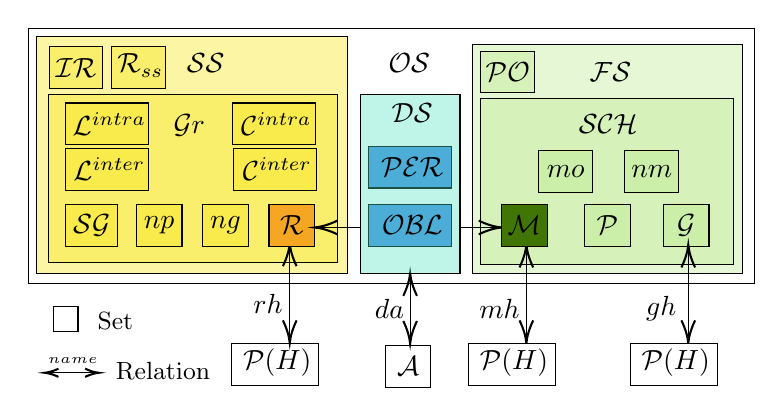
\begin{tikzpicture}[x=0.75pt,y=0.75pt,yscale=-1,xscale=1]
%uncomment if require: \path (0,1800); %set diagram left start at 0, and has height of 1800

%Shape: Rectangle [id:dp9341453924522656] 
\draw  [fill={rgb, 255:red, 255; green, 255; blue, 255 }  ,fill opacity=1 ] (160,44) -- (510,44) -- (510,167) -- (160,167) -- cycle ;
%Shape: Rectangle [id:dp4628140741854456] 
\draw  [fill={rgb, 255:red, 184; green, 233; blue, 134 }  ,fill opacity=0.34 ] (374,52) -- (504,52) -- (504,162) -- (374,162) -- cycle ;
%Shape: Rectangle [id:dp6461749357206974] 
\draw  [fill={rgb, 255:red, 184; green, 233; blue, 134 }  ,fill opacity=0.34 ] (378,78) -- (500,78) -- (500,158) -- (378,158) -- cycle ;
%Shape: Rectangle [id:dp47018118728898073] 
\draw  [fill={rgb, 255:red, 248; green, 231; blue, 28 }  ,fill opacity=0.4 ] (164,48) -- (314,48) -- (314,162) -- (164,162) -- cycle ;
%Straight Lines [id:da37904402438854] 
\draw    (400,150.31) -- (400,193.69) ;
\draw [shift={(400,195.69)}, rotate = 270] [color={rgb, 255:red, 0; green, 0; blue, 0 }  ][line width=0.75]    (10.93,-3.29) .. controls (6.95,-1.4) and (3.31,-0.3) .. (0,0) .. controls (3.31,0.3) and (6.95,1.4) .. (10.93,3.29)   ;
\draw [shift={(400,148.31)}, rotate = 90] [color={rgb, 255:red, 0; green, 0; blue, 0 }  ][line width=0.75]    (10.93,-3.29) .. controls (6.95,-1.4) and (3.31,-0.3) .. (0,0) .. controls (3.31,0.3) and (6.95,1.4) .. (10.93,3.29)   ;
%Straight Lines [id:da30557994145553513] 
\draw    (368,140) -- (386,140) ;
\draw [shift={(388,140)}, rotate = 180] [color={rgb, 255:red, 0; green, 0; blue, 0 }  ][line width=0.75]    (10.93,-3.29) .. controls (6.95,-1.4) and (3.31,-0.3) .. (0,0) .. controls (3.31,0.3) and (6.95,1.4) .. (10.93,3.29)   ;
%Shape: Rectangle [id:dp15689957472567295] 
\draw  [fill={rgb, 255:red, 248; green, 231; blue, 28 }  ,fill opacity=0.4 ] (169.56,76) -- (309.06,76) -- (309.06,157) -- (169.56,157) -- cycle ;
%Shape: Rectangle [id:dp6202366628126772] 
\draw  [fill={rgb, 255:red, 255; green, 255; blue, 255 }  ,fill opacity=1 ] (372,196) -- (414,196) -- (414,216) -- (372,216) -- cycle ;

%Shape: Rectangle [id:dp20067598884831228] 
\draw  [fill={rgb, 255:red, 248; green, 231; blue, 28 }  ,fill opacity=0.4 ] (212.06,129) -- (234.06,129) -- (234.06,149) -- (212.06,149) -- cycle ;

%Shape: Rectangle [id:dp5970765798398485] 
\draw  [fill={rgb, 255:red, 248; green, 231; blue, 28 }  ,fill opacity=0.4 ] (178.06,129) -- (203.06,129) -- (203.06,149) -- (178.06,149) -- cycle ;
%Shape: Rectangle [id:dp92237875722883] 
\draw  [fill={rgb, 255:red, 248; green, 231; blue, 28 }  ,fill opacity=0.4 ] (178.06,102) -- (218.06,102) -- (218.06,122) -- (178.06,122) -- cycle ;

%Shape: Rectangle [id:dp6591761395302378] 
\draw  [fill={rgb, 255:red, 248; green, 231; blue, 28 }  ,fill opacity=0.4 ] (178.06,80) -- (218.06,80) -- (218.06,100) -- (178.06,100) -- cycle ;

%Shape: Rectangle [id:dp11794703752595392] 
\draw  [fill={rgb, 255:red, 248; green, 231; blue, 28 }  ,fill opacity=0.4 ] (258.5,80) -- (298.5,80) -- (298.5,100) -- (258.5,100) -- cycle ;

%Shape: Rectangle [id:dp6557958558103134] 
\draw  [fill={rgb, 255:red, 248; green, 231; blue, 28 }  ,fill opacity=0.4 ] (259,102) -- (299,102) -- (299,122) -- (259,122) -- cycle ;

%Shape: Rectangle [id:dp8284992701408749] 
\draw  [fill={rgb, 255:red, 65; green, 117; blue, 5 }  ,fill opacity=1 ] (388,129) -- (410,129) -- (410,149) -- (388,149) -- cycle ;

%Shape: Rectangle [id:dp7066110016250453] 
\draw  [fill={rgb, 255:red, 248; green, 231; blue, 28 }  ,fill opacity=0.4 ] (244,129) -- (266,129) -- (266,149) -- (244,149) -- cycle ;

%Shape: Rectangle [id:dp4021333114319714] 
\draw  [fill={rgb, 255:red, 248; green, 231; blue, 28 }  ,fill opacity=0.4 ] (170.31,53) -- (195.69,53) -- (195.69,73) -- (170.31,73) -- cycle ;

%Shape: Rectangle [id:dp8476756388266236] 
\draw  [fill={rgb, 255:red, 248; green, 231; blue, 28 }  ,fill opacity=0.4 ] (200,53) -- (226,53) -- (226,73) -- (200,73) -- cycle ;

%Shape: Rectangle [id:dp07470576340681823] 
\draw  [fill={rgb, 255:red, 74; green, 144; blue, 226 }  ,fill opacity=1 ] (324,101) -- (364,101) -- (364,121) -- (324,121) -- cycle ;

%Shape: Rectangle [id:dp31407652093057714] 
\draw  [fill={rgb, 255:red, 74; green, 144; blue, 226 }  ,fill opacity=1 ] (324,129) -- (364,129) -- (364,149) -- (324,149) -- cycle ;

%Shape: Rectangle [id:dp053729126169398844] 
\draw  [fill={rgb, 255:red, 184; green, 233; blue, 134 }  ,fill opacity=0.34 ] (378,55) -- (404,55) -- (404,75) -- (378,75) -- cycle ;

%Shape: Rectangle [id:dp7720103442630182] 
\draw  [fill={rgb, 255:red, 184; green, 233; blue, 134 }  ,fill opacity=0.34 ] (405.94,103) -- (431.94,103) -- (431.94,123) -- (405.94,123) -- cycle ;

%Shape: Rectangle [id:dp3183552657000306] 
\draw  [fill={rgb, 255:red, 184; green, 233; blue, 134 }  ,fill opacity=0.34 ] (447.44,103) -- (473.44,103) -- (473.44,123) -- (447.44,123) -- cycle ;

%Shape: Rectangle [id:dp10802424702469593] 
\draw  [fill={rgb, 255:red, 184; green, 233; blue, 134 }  ,fill opacity=0.34 ] (466,129) -- (488,129) -- (488,149) -- (466,149) -- cycle ;

%Shape: Rectangle [id:dp16589412198505937] 
\draw  [fill={rgb, 255:red, 184; green, 233; blue, 134 }  ,fill opacity=0.34 ] (428,129) -- (450,129) -- (450,149) -- (428,149) -- cycle ;

%Shape: Rectangle [id:dp1270989692188249] 
\draw  [fill={rgb, 255:red, 255; green, 255; blue, 255 }  ,fill opacity=1 ] (258,196) -- (300,196) -- (300,216) -- (258,216) -- cycle ;

%Straight Lines [id:da40017392935840324] 
\draw    (286,149.69) -- (286,193.69) ;
\draw [shift={(286,195.69)}, rotate = 270] [color={rgb, 255:red, 0; green, 0; blue, 0 }  ][line width=0.75]    (10.93,-3.29) .. controls (6.95,-1.4) and (3.31,-0.3) .. (0,0) .. controls (3.31,0.3) and (6.95,1.4) .. (10.93,3.29)   ;
\draw [shift={(286,147.69)}, rotate = 90] [color={rgb, 255:red, 0; green, 0; blue, 0 }  ][line width=0.75]    (10.93,-3.29) .. controls (6.95,-1.4) and (3.31,-0.3) .. (0,0) .. controls (3.31,0.3) and (6.95,1.4) .. (10.93,3.29)   ;
%Shape: Rectangle [id:dp21027747628033966] 
\draw  [fill={rgb, 255:red, 245; green, 166; blue, 35 }  ,fill opacity=1 ] (276,129) -- (298,129) -- (298,149) -- (276,149) -- cycle ;

%Shape: Rectangle [id:dp5582162899072272] 
\draw  [fill={rgb, 255:red, 255; green, 255; blue, 255 }  ,fill opacity=1 ] (172,178) -- (184,178) -- (184,190) -- (172,190) -- cycle ;
%Straight Lines [id:da3472969066473863] 
\draw    (170,210) -- (192,210) ;
\draw [shift={(194,210)}, rotate = 180] [color={rgb, 255:red, 0; green, 0; blue, 0 }  ][line width=0.75]    (6.56,-1.97) .. controls (4.17,-0.84) and (1.99,-0.18) .. (0,0) .. controls (1.99,0.18) and (4.17,0.84) .. (6.56,1.97)   ;
\draw [shift={(168,210)}, rotate = 0] [color={rgb, 255:red, 0; green, 0; blue, 0 }  ][line width=0.75]    (6.56,-1.97) .. controls (4.17,-0.84) and (1.99,-0.18) .. (0,0) .. controls (1.99,0.18) and (4.17,0.84) .. (6.56,1.97)   ;
%Shape: Rectangle [id:dp07012270906311535] 
\draw  [fill={rgb, 255:red, 255; green, 255; blue, 255 }  ,fill opacity=1 ] (332,197) -- (354,197) -- (354,217) -- (332,217) -- cycle ;

%Straight Lines [id:da7534392810513293] 
\draw    (344,164) -- (344,194) ;
\draw [shift={(344,196)}, rotate = 270] [color={rgb, 255:red, 0; green, 0; blue, 0 }  ][line width=0.75]    (10.93,-3.29) .. controls (6.95,-1.4) and (3.31,-0.3) .. (0,0) .. controls (3.31,0.3) and (6.95,1.4) .. (10.93,3.29)   ;
\draw [shift={(344,162)}, rotate = 90] [color={rgb, 255:red, 0; green, 0; blue, 0 }  ][line width=0.75]    (10.93,-3.29) .. controls (6.95,-1.4) and (3.31,-0.3) .. (0,0) .. controls (3.31,0.3) and (6.95,1.4) .. (10.93,3.29)   ;
%Straight Lines [id:da4125176624573814] 
\draw    (320,140) -- (300,140) ;
\draw [shift={(298,140)}, rotate = 360] [color={rgb, 255:red, 0; green, 0; blue, 0 }  ][line width=0.75]    (10.93,-3.29) .. controls (6.95,-1.4) and (3.31,-0.3) .. (0,0) .. controls (3.31,0.3) and (6.95,1.4) .. (10.93,3.29)   ;
%Shape: Rectangle [id:dp005426842763594397] 
\draw  [fill={rgb, 255:red, 80; green, 227; blue, 194 }  ,fill opacity=0.36 ] (320,76) -- (368,76) -- (368,162) -- (320,162) -- cycle ;
%Straight Lines [id:da9128713017721406] 
\draw    (478,150.31) -- (478,193.69) ;
\draw [shift={(478,195.69)}, rotate = 270] [color={rgb, 255:red, 0; green, 0; blue, 0 }  ][line width=0.75]    (10.93,-3.29) .. controls (6.95,-1.4) and (3.31,-0.3) .. (0,0) .. controls (3.31,0.3) and (6.95,1.4) .. (10.93,3.29)   ;
\draw [shift={(478,148.31)}, rotate = 90] [color={rgb, 255:red, 0; green, 0; blue, 0 }  ][line width=0.75]    (10.93,-3.29) .. controls (6.95,-1.4) and (3.31,-0.3) .. (0,0) .. controls (3.31,0.3) and (6.95,1.4) .. (10.93,3.29)   ;
%Shape: Rectangle [id:dp7604827971406838] 
\draw  [fill={rgb, 255:red, 255; green, 255; blue, 255 }  ,fill opacity=1 ] (450,196) -- (492,196) -- (492,216) -- (450,216) -- cycle ;



% Text Node
\draw (465,179) node   [align=left] {$gh$};
% Text Node
\draw (181.5,204) node  [font=\tiny] [align=left] {$name$};
% Text Node
\draw (334,179) node   [align=left] {$da$};
% Text Node
\draw (222,207) node  [font=\footnotesize] [align=left] {\begin{minipage}[lt]{29.67pt}\setlength\topsep{0pt}
\begin{center}
{\small Relation}
\end{center}

\end{minipage}};
% Text Node
\draw (202,185) node  [font=\footnotesize] [align=left] {\begin{minipage}[lt]{13.75pt}\setlength\topsep{0pt}
\begin{center}
{\small Set}
\end{center}

\end{minipage}};
% Text Node
\draw (343.5,61) node   [align=left] {$\mathcal{OS}$};
% Text Node
\draw (190.56,139) node   [align=left] {$\mathcal{SG}$};
% Text Node
\draw (345,85) node   [align=left] {$\mathcal{DS}$};
% Text Node
\draw (245.5,61) node   [align=left] {$\mathcal{SS}$};
% Text Node
\draw (387,179) node   [align=left] {$mh$};
% Text Node
\draw (275.5,177) node   [align=left] {$rh$};
% Text Node
\draw (237.56,91) node   [align=left] {$\mathcal{G}r$};
% Text Node
\draw (440.5,65) node   [align=left] {$\mathcal{FS}$};
% Text Node
\draw (439.44,90) node   [align=left] {$\mathcal{SCH}$};
% Text Node
\draw (472,205) node   [align=left] {$\mathcal{P}(H)$};
% Text Node
\draw (343,207) node   [align=left] {$\mathcal{A}$};
% Text Node
\draw (287,139) node   [align=left] {$\mathcal{R}$};
% Text Node
\draw (280,205) node   [align=left] {$\mathcal{P}(H)$};
% Text Node
\draw (439,139) node   [align=left] {$\mathcal{P}$};
% Text Node
\draw (477,139) node   [align=left] {$\mathcal{G}$};
% Text Node
\draw (460.44,113) node   [align=left] {$nm$};
% Text Node
\draw (418.94,113) node   [align=left] {$mo$};
% Text Node
\draw (391,65) node   [align=left] {$\mathcal{PO}$};
% Text Node
\draw (345,139) node   [align=left] {$\mathcal{OBL}$};
% Text Node
\draw (345,111) node   [align=left] {$\mathcal{PER}$};
% Text Node
\draw (214,62) node   [align=left] {$\mathcal{R}_{ss}$};
% Text Node
\draw (183,63) node   [align=left] {$\mathcal{IR}$};
% Text Node
\draw (255,139) node   [align=left] {$\mathnormal{ng}$};
% Text Node
\draw (399,139) node   [align=left] {$\mathcal{M}$};
% Text Node
\draw (280,112) node   [align=left] {$\mathcal{C}^{inter}$};
% Text Node
\draw (279.5,90) node   [align=left] {$\mathcal{C}^{intra}$};
% Text Node
\draw (199.06,90) node   [align=left] {$\mathcal{L}^{intra}$};
% Text Node
\draw (199.06,112) node   [align=left] {$\mathcal{L}^{inter}$};
% Text Node
\draw (223.06,139) node   [align=left] {$np$};
% Text Node
\draw (394,205) node   [align=left] {$\mathcal{P}(H)$};


\end{tikzpicture}
    \caption{An view of relations between organizational specification to history subsets}
    \label{fig:PRAHOM_osm_rels}
\end{figure}

\



This idea led to the following additional theoretical tools we propose as prior requirements.

\

% \noindent \textbf{Observable policy} \quad We propose to represent a role $\rho \in \mathcal{R}$ in MARL formalism by introducing an \textbf{observable policy} $\pi_{\rho} \in \Pi, \pi_{\rho} = rcnt \circ play_l$ so that a policy generates histories (of $l \in \mathbb{N}$ length) $h \in H$ that belong to the agent observable/expected history subset $H_{\rho}$. The relation $rcnt: \mathcal{P}(H) \rightarrow \Pi_{\mathcal{R}}$ enables reconstructing an observable policy based upon collected histories. The relation $play_l = play: \Pi \times \mathbb{N} \rightarrow \mathcal{P}(H)$ enables generating histories (of $l \in \mathbb{N}$ length) according to a policy. For a representative amount of histories in $H = play_l(\pi)$, $\pi_{\mathcal{R}} = rcnt(H)$ is considered to be an approximation of $\pi$.
% Unlike black-box policies, the mapping of an observable policy associating couples (history, observation) to action is explicit.

% \

\noindent \textbf{Observable policy constraint} \quad We propose to represent the constraints of policy $\pi \in \Pi$ by introducing an \textbf{observable policy constraint} $\pi_c: H times \Omega \rightarrow \mathcal{P}(A)$. $\pi_c$ indicates the actions an agent's policy should be allowed to choose among when it receives an observation at each step. We denote, $bld_{opc}: \mathcal{P}(H) \rightarrow \Pi_c$ the relation that enables creating an observable policy constraint from a given history subset.

\

\noindent \textbf{Observable reward function} \quad We propose to represent a goal $g \in \mathcal{G}$ in MARL formalism by introducing an \textbf{observable reward function} $R_{g}: H \rightarrow \mathbb{R} = bld_{rwf}(H_g) = \{(h, dist(H_g,h)), h \in H\}$ so that a history generated by an agent $h \in H$ be associated with a positive reward if it belongs to the observable/expected $H_g$ or negative otherwise. The relation $dist: H \times H \rightarrow \mathbb{R}$ associate a real number indicating how close a generated history belong to a given history subset. The relation $bld_{rwf}: H \rightarrow R$ generates an observable reward function from a reference given history subset.
A mission $m \in \mathcal{M}$ containing goals $\mathcal{G} = mo(m) = \{g_i \in \mathcal{G}\}$ is represented as $R_m: H \rightarrow \mathbb{R} = comb(\{bld_{rwf}(H_g), g \in G, H_g = gh(g) \subset H\})$. The relation $comb: \mathcal{M} \times \mathcal{P}(\mathcal{G}) \rightarrow R_{\mathcal{M}}$ combines all observable reward function of each goal into a single observable reward function.

\

In the remainder of this section, we give an overview of the theory we propose to implement the features $(G_E.F_S)$, $(G_E.F_F)$, $(G_E.F_D)$ into the proposed $PRAHOM_E$ algorithm presented in \autoref{alg:PRAHOM-E}
to get OS from histories. We also briefly depict the proposed theory for implementing the features $(G_A.F_S)$, $(G_A.F_F)$, $(G_A.F_D)$ into the proposed $PRAHOM_A$ algorithm presented in \autoref{alg:PRAHOM-A} to constrain policies according to OS.

Then, PRAHOM is a synthesis of these two algorithms presented in \autoref{alg:PRAHOM}. It first consists in training a joint-policy $\pi_{joint}$ in the given environment under organizational constraints. It enables getting the joint-policies that reach the given expectancy. Then, each of these joint-policies is played within differently generated environments to get all the joint-histories $sh{joint,i,s}$. Finally, these joint-histories are analyzed to infer the associated organizational specifications enriching known relations\footnotemark[1].

\footnotetext[1]{Additional information are provided in addition to developed code in \url{https://github.com/julien6/omarl_experiments}.}

\RestyleAlgo{ruled}
\SetKwComment{Comment}{// }{}

\begin{algorithm}[hbt!]
    \caption{\emph{PRAHOM}}\label{alg:PRAHOM}

    \KwData{$d \in D$, Dec-POMDP to solve}
    \KwData{$ep_{max} \in \mathbb{N}$, maximum number of episodes}
    \KwData{$it_{max} \in \mathbb{N}$, maximum number of iteration}
    \KwData{$step_{max} \in \mathbb{N}$, maximum number of step per episode}
    \KwData{$s \in \mathbb{R}$, cumulative reward expectancy}
    \KwData{$sfh: \mathcal{R} \cup \mathcal{G} \rightarrow \mathcal{P}(H)$, the bijection from role/goals to history subsets}
    \KwData{$da: \mathcal{D} \rightarrow \mathcal{P}(A)$, the bijection from permission/obligation to agents}
    \KwData{$marl\_alg: \Pi_{joint} \times H_{joint} \times \mathbb{R}^{step_{max}} \rightarrow \Pi_{joint}$, algorithm to train from histories and rewards}

    \KwResult{$(\pi_{joint,i,s} \in \Pi_{joint}, os_{i,s} \in \mathcal{OS})$, trained policies and org. specs.}

    \Comment{Init policy}

    $\pi_{joint,i,init} = marl\_alg.init()$

    \Comment{Training under org. specs. constraints}

    $\pi_{joint,i,s} = \mathbf{PRAHOM_A}(sfh,da,\pi_{joint,i,init},s,marl\_alg\dots)$

    \Comment{Get joint-histories from the trained $\pi_{joint,i,s}$}
    $H_{joint,i,s} \in \mathcal{P}(H_{joint}) = play(ep_{max}, s\pi_{joint,i,s})$

    \Comment{Get org. specs. from these joint-histories}
    $os_{i,s} = \mathbf{PRAHOM_E}(H_{joint,i,s},da,sfh\dots)$

\end{algorithm}


\subsection{\textbf{Inferring OS from histories: $PRAHOM_E$}}

% \paragraph{\textbf{$(\mathbf{G_E.F_S})$: Inferring SS}}

% \paragraph{\textbf{$(\mathbf{G_E.F_F})$: Inferring FS}}

% \paragraph{\textbf{$(\mathbf{G_E.F_D})$: Inferring DS}}

\noindent The underlying principle of $PRAHOM_E$ presented \autoref{alg:PRAHOM-E} firstly relies on the proposed \emph{Knowledge-based Organizational Specification Identification Approach} (KOSIA) that uses currently known $sfh$ to identify some roles, missions (from goals), and permissions/obligation. These organizational specifications can be completed from other linked known organizational specifications such as \emph{link}, \emph{compatibilities}, \emph{plans}\dots. % KOSIA is aimed to be relevant when knowledge of the relations between histories and organizational specifications is significant enough to be used generally.
% For instance, we implemented KOSIA as a pattern-matching engine finding similar joint-histories $Im(sfh)$ to a given one hence finding the associated organizational specifications.
%
Otherwise, if it is not possible to get all known associated organizational specifications, the proposed \emph{General Organizational Specification Inference Approach} (GOSIA) suggests an empirical approach to infer the rest of them.
GOSIA is based on some proposed definitions for each $\mathcal{M}OISE^+$ organizational specification regarding joint-histories or other organizational specifications, to use suggested specific statistical, unsupervised learning techniques to infer them incrementally. GOSIA runs through five steps that presented hereafter.
% The \autoref{fig:gosia_illustrative_view} summarizes the five steps of GOSIA (represented as arrow labels in \autoref{fig:gosia_illustrative_view}) that are detailed below.
%
\paragraph{1) Infer roles and their inheritance}

We propose a role $\rho$ is defined as a policy whose the associated histories of agents having adopted it all contain a common discontinuous sequence. We proposed a role $\rho_2$ inherits $\rho_2$ if the common discontinuous sequence of the histories associated with $\rho_2$ is also contained in the $\rho_1$'s one.
From these definitions, GOSIA leverages hierarchical sequence clustering to find the longest common discontinuous sequences among agent's histories. Results can represented as a dendrogram. It enables inferring roles and inheritance relations, their respective relation with histories, and the current agents as well.

\paragraph{2) Infer possible organizations}

We propose an organization is linked to only one set of all instantiable roles sharing closely similar inheritance relations. Indeed, considering two joint-histories from trained joint-policies $H_{joint,i,s,1}$ and $H_{joint,i,s,2}$, even though both achieve a goal relying on the roles $\mathcal{R}_{ss,1}$ and $\mathcal{R}_{ss,2}$ may be far from other. For instance, their roles may not use the same responsibility distribution.
GOSIA uses a K-means algorithm to get the $q$ clusters of the vectorized $\mathcal{IR}_{i}$ considered as organizations. The roles in the same cluster share the inheritance relations of the K-means' centroid $\mathcal{IR}_j$. Indeed, they are representative general roles regarding all the similar roles adopted by agents of the same organization over all joint-histories.
For the next steps, only one chosen organization and its related joint-histories are considered. When it exists it chooses an organization close to KOSIA's one.

\paragraph{3) Infer links and sub-groups}

We propose two agents have a \emph{social impact link} $(ag_1,ag_2, \kappa, \delta, f)$ with $h_1$ associated with $ag_1$ and $h_2$ associated with $ag_2$ if a sequence $h_{1,s}$ in $h_1$ is correlated at a $\kappa \in [0,1]$ index to another sequence $h_{2,s}$ in $h_2$ positioned at a relative delay $\delta \in [0,1]$ after the beginning of $h_{1,s}$, and these two correlated sequences are $f$ frequently present among all joint-policies.
We consider two agents to be in the same group if there is a social impact link such as $f \geq 0.9$. Considering that $\kappa$ indicates the likeliness of an agent' sequence to impact another one and that $\delta$ indicates the receiver's reactivity, we consider:
\begin{itemize}
    \item an acquaintance link $(ag_1,ag_2,acq)$ is defined if there is a social impact link with $\kappa \geq 0.1$, $\delta \geq 0$, $f \geq 0$;
    \item a communication link $(ag_1,ag_2,com)$ is defined if there is a social impact link with $\kappa \geq 0.3$, $\delta \geq 0$, $f \geq 0$;
    \item an authority link $(ag_1,ag_2,aut)$ is defined if there is a social impact link with $\kappa \geq 0.9$, $\delta \geq 0.5$, $f \geq 0$.
\end{itemize}
% TODO: Generaliser à plusieurs agents ou le dire en tant que limitation
GOSIA uses empirical techniques to compute a graph of the social impact links between agents. Frequency enables determining clusters as agents' groups and their associated roles. It enables inferring the acquaintance, communication, and authority links between roles. From the information concerning roles associated with groups, it is possible to infer whether links are intra-group or inter-group.

\paragraph{4) Infer goals, plans, and missions}

We propose a sub-goal/goal is a set of common states that are reached following the histories of the successful agents.
For each joint-history GOSIA computes the state transition graph that is merged into a general one. Measuring the distance between two vectorized states within K-means enables finding the clusters of trajectories that some agents may follow. Then, we sampled some sets of states for each trajectory as goals. For instance, one may choose the narrowest set of states in which agents collectively seem to transition at some point to achieve their goal. Otherwise, a balanced sampling over lower variance trajectories could be made. Knowing what goal belongs to what trajectory, GOSIA infers plans for choice and sequence only.

This enables getting goals and plans at a global state but these goals could be indeed split into specific goals for each sub-group and agent. To do this, GOSIA conducts the same process replacing the states with the observations of the agents in the same sub-group for sub-groups, and observations for agents.

We propose a mission as the set of sub-goals one or several agents are achieving.
Knowing what shared goals are achieved by agents, GOSIA determines some sets of representative goals as missions.

\paragraph{5) Infer compatibilities, obligations, permissions, and cardinalities}

We propose an obligation is when an agent playing role $\rho$ is achieving a mission's goals and no other one at some time constraints while an obligation is when an agent playing role $\rho$ may achieve some other ones at some time constraints.
GOSIA determines what agents' are associated with what mission and if they are restricted to some hence these are obligations or just permission

We propose a compatibility $(\rho_1,\rho_2)$ is defined if an agent playing a history associated with $\rho_1$ in a joint-history also plays a history associated with $\rho_2$ in another joint-history. If this change operates only in the same group, then it is intra-group. Else it is inter-group.

Finally, by counting the number of agents playing a role in each joint-history, each role's cardinality is computed. Similarly, GOSIA computes each sub-group's cardinality counting the inferred ones.

\RestyleAlgo{ruled}
\SetKwComment{Comment}{// }{}

\begin{algorithm}[hbt!]
    \caption{$PRAHOM_E$}\label{alg:PRAHOM-E}

    \KwData{$da: \mathcal{D} \rightarrow \mathcal{P}(A)$, the bijection from permission/obligation to agents}

    \KwData{$sfh: \mathcal{R} \cup \mathcal{G} \rightarrow \mathcal{P}(H)$, the bijection from role/goals to history subsets}

    \KwData{$H_{joint,i,s}$, joint-histories to be analyzed}

    \KwResult{$os \subseteq OS$, associated organization specifications}

    \Comment{KOSIA: identify from known relations}

    $os = \mathbf{KOSIA}(da, fsh, H_{joint,i,s},\dots)$

    \uIf{any org. spec. $\in os$ is $\emptyset$}{

        \Comment{GOSIA: infer from OS definitions to complete identified OS}

        $os = \mathbf{GOSIA}(os, da, fsh, H_{joint,i},\dots)$

    }

\end{algorithm}

% \begin{figure*}[h!]
%     \centering
%     


\tikzset{every picture/.style={line width=0.75pt}} %set default line width to 0.75pt        

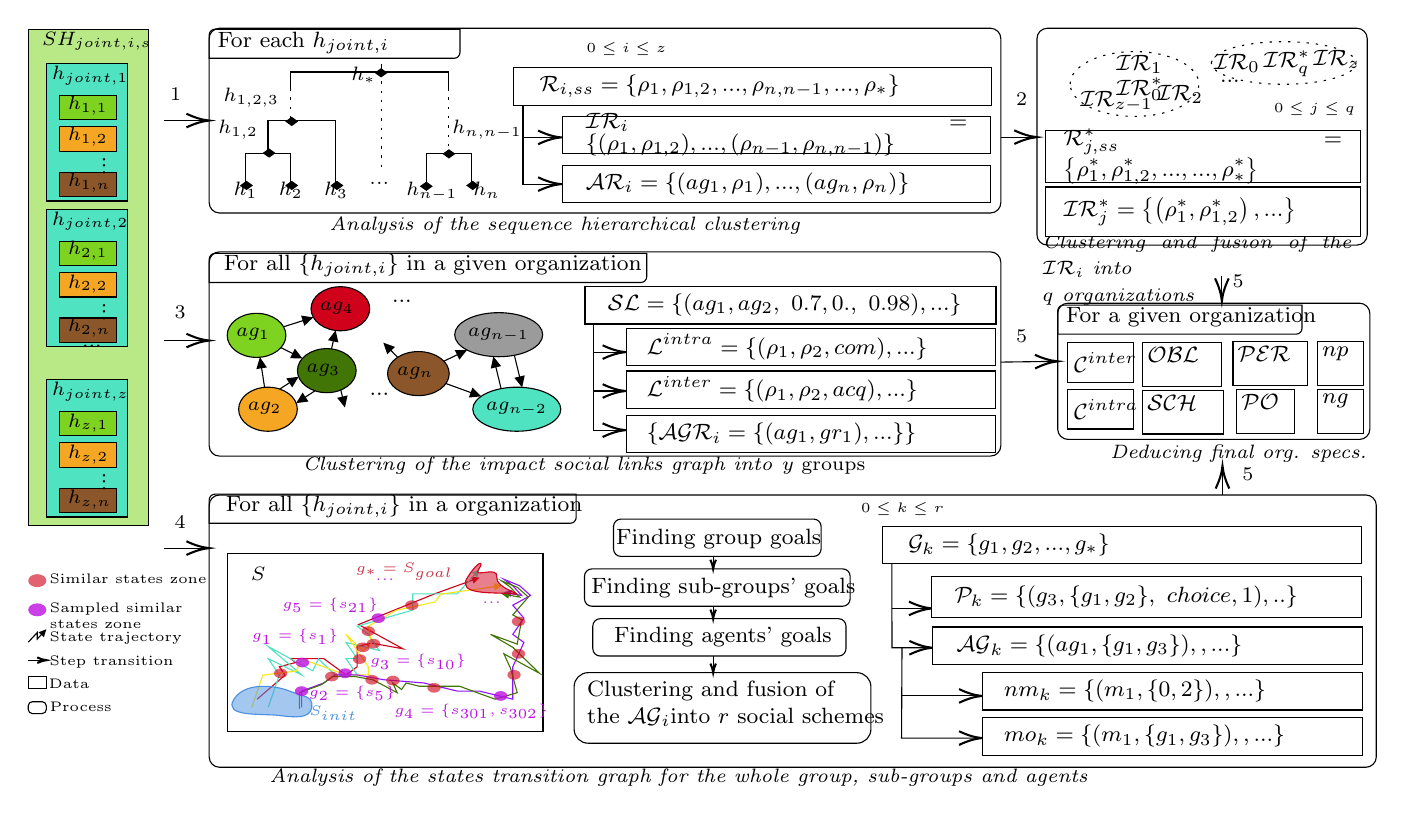
\begin{tikzpicture}[x=0.75pt,y=0.75pt,yscale=-1,xscale=1]
%uncomment if require: \path (0,1523); %set diagram left start at 0, and has height of 1523

%Shape: Rectangle [id:dp8437675271367469] 
\draw  [fill={rgb, 255:red, 255; green, 255; blue, 255 }  ,fill opacity=1 ] (95.9,1122.51) -- (248,1122.51) -- (248,1208.4) -- (95.9,1208.4) -- cycle ;
%Straight Lines [id:da030048051476729842] 
\draw [color={rgb, 255:red, 208; green, 2; blue, 27 }  ,draw opacity=1 ]   (214.57,1135.24) -- (196.18,1141.89) -- (159.16,1156.81) -- (180.58,1168.52) -- (165.43,1165.76) -- (158.48,1167.41) -- (158.48,1177.17) -- (153.95,1180.47) -- (153.12,1181.07) -- (150.55,1179.2) -- (142.41,1173.26) -- (126.34,1173.26) -- (128.9,1175.13) -- (120.99,1177.17) -- (123.75,1181.19) -- (110.28,1192.78) ;
\draw [shift={(217.39,1134.22)}, rotate = 160.12] [fill={rgb, 255:red, 208; green, 2; blue, 27 }  ,fill opacity=1 ][line width=0.08]  [draw opacity=0] (3.57,-1.72) -- (0,0) -- (3.57,1.72) -- cycle    ;
%Straight Lines [id:da3391044780146215] 
\draw [color={rgb, 255:red, 80; green, 227; blue, 194 }  ,draw opacity=1 ]   (215.37,1132.53) -- (206.68,1142.03) -- (185.26,1142.03) -- (185.26,1149.84) -- (158.48,1157.65) -- (163.83,1161.55) -- (169.19,1169.36) -- (153.12,1165.46) -- (158.48,1173.26) -- (153.12,1173.26) -- (158.48,1181.07) -- (147.77,1181.07) -- (139.84,1173.34) -- (137.05,1179.12) -- (115.63,1167.41) -- (131.7,1181.07) -- (115.63,1173.26) -- (120.99,1181.07) -- (115.63,1196.69) ;
\draw [shift={(217.39,1130.32)}, rotate = 132.45] [fill={rgb, 255:red, 80; green, 227; blue, 194 }  ,fill opacity=1 ][line width=0.08]  [draw opacity=0] (3.57,-1.72) -- (0,0) -- (3.57,1.72) -- cycle    ;
%Straight Lines [id:da7194825305170893] 
\draw [color={rgb, 255:red, 248; green, 231; blue, 28 }  ,draw opacity=1 ]   (225.13,1138.53) -- (198.73,1142.15) -- (195.97,1145.94) -- (177.3,1149.96) -- (163.83,1157.65) -- (165.43,1165.76) -- (161.24,1169.48) -- (153.12,1161.55) -- (163.83,1177.17) -- (163.83,1181.07) -- (153.12,1181.07) -- (131.89,1173.46) -- (129.1,1179.24) -- (113.04,1181.19) -- (107.68,1196.81) ;
\draw [shift={(228.1,1138.13)}, rotate = 172.2] [fill={rgb, 255:red, 248; green, 231; blue, 28 }  ,fill opacity=1 ][line width=0.08]  [draw opacity=0] (3.57,-1.72) -- (0,0) -- (3.57,1.72) -- cycle    ;
%Straight Lines [id:da36953350175148314] 
\draw [color={rgb, 255:red, 144; green, 19; blue, 254 }  ,draw opacity=1 ]   (232.12,1141.79) -- (237.74,1142.81) -- (233.46,1138.13) -- (229.17,1135) -- (236.76,1138.13) -- (242.03,1142.81) -- (233.46,1147.5) -- (238.81,1153.74) -- (233.46,1161.55) -- (238.81,1165.46) -- (233.46,1177.17) -- (233.46,1192.78) -- (217.39,1188.88) -- (206.68,1188.88) -- (200.88,1187.47) -- (197.82,1186.73) -- (193.47,1185.67) -- (190.61,1184.97) -- (179.86,1184.1) -- (171.33,1183.41) -- (167.13,1182.65) -- (158.48,1181.07) -- (147.77,1181.07) -- (142.41,1184.97) -- (131.7,1188.88) -- (131.7,1196.69) ;
\draw [shift={(229.17,1141.25)}, rotate = 10.33] [fill={rgb, 255:red, 144; green, 19; blue, 254 }  ,fill opacity=1 ][line width=0.08]  [draw opacity=0] (3.57,-1.72) -- (0,0) -- (3.57,1.72) -- cycle    ;
%Straight Lines [id:da8314531084394159] 
\draw [color={rgb, 255:red, 65; green, 117; blue, 5 }  ,draw opacity=1 ]   (231.05,1142.57) -- (236.67,1143.59) -- (232.39,1138.91) -- (228.1,1135.78) -- (235.69,1138.91) -- (240.95,1143.59) -- (233.46,1152.18) -- (237.74,1154.52) -- (235.6,1166.24) -- (222.75,1161.55) -- (233.46,1167.8) -- (246.31,1180.29) -- (229.17,1170.92) -- (232.39,1177.95) -- (235.6,1189.66) -- (224.89,1192.78) -- (207.75,1186.54) -- (194.9,1186.54) -- (188.47,1186.54) -- (182.04,1184.97) -- (179.9,1188.1) -- (175.62,1184.97) -- (177.76,1189.66) -- (166.06,1183.43) -- (157.41,1181.85) -- (146.69,1181.85) -- (141.34,1185.76) -- (130.63,1189.66) -- (130.63,1197.47) ;
\draw [shift={(228.1,1142.03)}, rotate = 10.33] [fill={rgb, 255:red, 65; green, 117; blue, 5 }  ,fill opacity=1 ][line width=0.08]  [draw opacity=0] (3.57,-1.72) -- (0,0) -- (3.57,1.72) -- cycle    ;
%Shape: Ellipse [id:dp9217980363047418] 
\draw  [draw opacity=0][fill={rgb, 255:red, 208; green, 2; blue, 27 }  ,fill opacity=0.62 ] (118.39,1180.29) .. controls (118.39,1179) and (119.83,1177.95) .. (121.61,1177.95) .. controls (123.38,1177.95) and (124.82,1179) .. (124.82,1180.29) .. controls (124.82,1181.58) and (123.38,1182.63) .. (121.61,1182.63) .. controls (119.83,1182.63) and (118.39,1181.58) .. (118.39,1180.29) -- cycle ;
%Shape: Ellipse [id:dp9560113901350078] 
\draw  [draw opacity=0][fill={rgb, 255:red, 208; green, 2; blue, 27 }  ,fill opacity=0.62 ] (162.39,1183.43) .. controls (162.39,1182.13) and (163.83,1181.09) .. (165.6,1181.09) .. controls (167.38,1181.09) and (168.82,1182.13) .. (168.82,1183.43) .. controls (168.82,1184.72) and (167.38,1185.77) .. (165.6,1185.77) .. controls (163.83,1185.77) and (162.39,1184.72) .. (162.39,1183.43) -- cycle ;
%Shape: Ellipse [id:dp5873799962452881] 
\draw  [draw opacity=0][fill={rgb, 255:red, 208; green, 2; blue, 27 }  ,fill opacity=0.62 ] (233,1170.92) .. controls (233,1169.63) and (234.44,1168.58) .. (236.22,1168.58) .. controls (237.99,1168.58) and (239.43,1169.63) .. (239.43,1170.92) .. controls (239.43,1172.21) and (237.99,1173.26) .. (236.22,1173.26) .. controls (234.44,1173.26) and (233,1172.21) .. (233,1170.92) -- cycle ;
%Shape: Ellipse [id:dp5660506421902496] 
\draw  [draw opacity=0][fill={rgb, 255:red, 208; green, 2; blue, 27 }  ,fill opacity=0.62 ] (192.3,1187.32) .. controls (192.3,1186.02) and (193.74,1184.97) .. (195.51,1184.97) .. controls (197.29,1184.97) and (198.73,1186.02) .. (198.73,1187.32) .. controls (198.73,1188.61) and (197.29,1189.66) .. (195.51,1189.66) .. controls (193.74,1189.66) and (192.3,1188.61) .. (192.3,1187.32) -- cycle ;
%Shape: Ellipse [id:dp042659050023868605] 
\draw  [draw opacity=0][fill={rgb, 255:red, 208; green, 2; blue, 27 }  ,fill opacity=0.62 ] (233,1155.3) .. controls (233,1154.01) and (234.44,1152.96) .. (236.22,1152.96) .. controls (237.99,1152.96) and (239.43,1154.01) .. (239.43,1155.3) .. controls (239.43,1156.6) and (237.99,1157.65) .. (236.22,1157.65) .. controls (234.44,1157.65) and (233,1156.6) .. (233,1155.3) -- cycle ;
%Shape: Ellipse [id:dp5012921217565263] 
\draw  [draw opacity=0][fill={rgb, 255:red, 208; green, 2; blue, 27 }  ,fill opacity=0.62 ] (158.02,1167.8) .. controls (158.02,1166.5) and (159.46,1165.46) .. (161.24,1165.46) .. controls (163.01,1165.46) and (164.45,1166.5) .. (164.45,1167.8) .. controls (164.45,1169.09) and (163.01,1170.14) .. (161.24,1170.14) .. controls (159.46,1170.14) and (158.02,1169.09) .. (158.02,1167.8) -- cycle ;
%Shape: Ellipse [id:dp09659905080826858] 
\draw  [draw opacity=0][fill={rgb, 255:red, 208; green, 2; blue, 27 }  ,fill opacity=0.62 ] (181.59,1147.5) .. controls (181.59,1146.2) and (183.03,1145.15) .. (184.8,1145.15) .. controls (186.58,1145.15) and (188.02,1146.2) .. (188.02,1147.5) .. controls (188.02,1148.79) and (186.58,1149.84) .. (184.8,1149.84) .. controls (183.03,1149.84) and (181.59,1148.79) .. (181.59,1147.5) -- cycle ;
%Shape: Ellipse [id:dp1880200695236467] 
\draw  [draw opacity=0][fill={rgb, 255:red, 189; green, 16; blue, 224 }  ,fill opacity=0.8 ] (149.46,1180.29) .. controls (149.46,1179) and (150.89,1177.95) .. (152.67,1177.95) .. controls (154.44,1177.95) and (155.88,1179) .. (155.88,1180.29) .. controls (155.88,1181.58) and (154.44,1182.63) .. (152.67,1182.63) .. controls (150.89,1182.63) and (149.46,1181.58) .. (149.46,1180.29) -- cycle ;
%Shape: Ellipse [id:dp9871531520887487] 
\draw  [draw opacity=0][fill={rgb, 255:red, 208; green, 2; blue, 27 }  ,fill opacity=0.62 ] (156.42,1173.46) .. controls (156.42,1172.16) and (157.86,1171.12) .. (159.63,1171.12) .. controls (161.41,1171.12) and (162.84,1172.16) .. (162.84,1173.46) .. controls (162.84,1174.75) and (161.41,1175.8) .. (159.63,1175.8) .. controls (157.86,1175.8) and (156.42,1174.75) .. (156.42,1173.46) -- cycle ;
%Shape: Ellipse [id:dp8654501517781246] 
\draw  [draw opacity=0][fill={rgb, 255:red, 208; green, 2; blue, 27 }  ,fill opacity=0.62 ] (163.11,1166.04) .. controls (163.11,1164.75) and (164.55,1163.7) .. (166.33,1163.7) .. controls (168.1,1163.7) and (169.54,1164.75) .. (169.54,1166.04) .. controls (169.54,1167.33) and (168.1,1168.38) .. (166.33,1168.38) .. controls (164.55,1168.38) and (163.11,1167.33) .. (163.11,1166.04) -- cycle ;
%Shape: Ellipse [id:dp28595404701705673] 
\draw  [draw opacity=0][fill={rgb, 255:red, 208; green, 2; blue, 27 }  ,fill opacity=0.62 ] (172.48,1183.8) .. controls (172.48,1182.51) and (173.92,1181.46) .. (175.7,1181.46) .. controls (177.47,1181.46) and (178.91,1182.51) .. (178.91,1183.8) .. controls (178.91,1185.1) and (177.47,1186.15) .. (175.7,1186.15) .. controls (173.92,1186.15) and (172.48,1185.1) .. (172.48,1183.8) -- cycle ;
%Shape: Ellipse [id:dp2762324596061283] 
\draw  [draw opacity=0][fill={rgb, 255:red, 189; green, 16; blue, 224 }  ,fill opacity=0.8 ] (224.43,1191.22) .. controls (224.43,1189.93) and (225.87,1188.88) .. (227.65,1188.88) .. controls (229.42,1188.88) and (230.86,1189.93) .. (230.86,1191.22) .. controls (230.86,1192.51) and (229.42,1193.56) .. (227.65,1193.56) .. controls (225.87,1193.56) and (224.43,1192.51) .. (224.43,1191.22) -- cycle ;
%Shape: Ellipse [id:dp06377078584077789] 
\draw  [draw opacity=0][fill={rgb, 255:red, 208; green, 2; blue, 27 }  ,fill opacity=0.62 ] (230.86,1181.07) .. controls (230.86,1179.78) and (232.3,1178.73) .. (234.08,1178.73) .. controls (235.85,1178.73) and (237.29,1179.78) .. (237.29,1181.07) .. controls (237.29,1182.36) and (235.85,1183.41) .. (234.08,1183.41) .. controls (232.3,1183.41) and (230.86,1182.36) .. (230.86,1181.07) -- cycle ;
%Shape: Ellipse [id:dp8278424167241658] 
\draw  [draw opacity=0][fill={rgb, 255:red, 189; green, 16; blue, 224 }  ,fill opacity=0.8 ] (128.9,1175.13) .. controls (128.9,1173.83) and (130.34,1172.78) .. (132.11,1172.78) .. controls (133.89,1172.78) and (135.33,1173.83) .. (135.33,1175.13) .. controls (135.33,1176.42) and (133.89,1177.47) .. (132.11,1177.47) .. controls (130.34,1177.47) and (128.9,1176.42) .. (128.9,1175.13) -- cycle ;
%Shape: Ellipse [id:dp43060811492983575] 
\draw  [draw opacity=0][fill={rgb, 255:red, 208; green, 2; blue, 27 }  ,fill opacity=0.62 ] (160.62,1159.99) .. controls (160.62,1158.7) and (162.06,1157.65) .. (163.83,1157.65) .. controls (165.61,1157.65) and (167.05,1158.7) .. (167.05,1159.99) .. controls (167.05,1161.28) and (165.61,1162.33) .. (163.83,1162.33) .. controls (162.06,1162.33) and (160.62,1161.28) .. (160.62,1159.99) -- cycle ;
%Shape: Ellipse [id:dp797522001890842] 
\draw  [draw opacity=0][fill={rgb, 255:red, 189; green, 16; blue, 224 }  ,fill opacity=0.8 ] (165.44,1153.74) .. controls (165.44,1152.45) and (166.88,1151.4) .. (168.65,1151.4) .. controls (170.43,1151.4) and (171.87,1152.45) .. (171.87,1153.74) .. controls (171.87,1155.04) and (170.43,1156.09) .. (168.65,1156.09) .. controls (166.88,1156.09) and (165.44,1155.04) .. (165.44,1153.74) -- cycle ;
%Shape: Polygon Curved [id:ds4655017653667326] 
\draw  [color={rgb, 255:red, 74; green, 144; blue, 226 }  ,draw opacity=1 ][fill={rgb, 255:red, 74; green, 144; blue, 226 }  ,fill opacity=0.5 ] (99.11,1192.78) .. controls (102.28,1187.79) and (108.53,1186.39) .. (114.46,1186.58) .. controls (118.95,1186.73) and (123.26,1187.78) .. (125.89,1188.88) .. controls (132,1191.42) and (137.46,1191.03) .. (136.6,1196.69) .. controls (135.74,1202.35) and (128.78,1201.57) .. (120.53,1200.59) .. controls (112.29,1199.61) and (93.54,1201.57) .. (99.11,1192.78) -- cycle ;
%Shape: Polygon Curved [id:ds019315332146999653] 
\draw  [color={rgb, 255:red, 208; green, 2; blue, 27 }  ,draw opacity=1 ][fill={rgb, 255:red, 208; green, 2; blue, 27 }  ,fill opacity=0.5 ] (211.58,1134.22) .. controls (217.15,1125.44) and (219.91,1125.99) .. (216.94,1130.32) .. controls (213.97,1134.65) and (226.58,1128.27) .. (225.72,1133.93) .. controls (224.86,1139.59) and (241.25,1143.01) .. (233,1142.03) .. controls (224.76,1141.06) and (206.01,1143.01) .. (211.58,1134.22) -- cycle ;
%Shape: Ellipse [id:dp012062721326329351] 
\draw  [draw opacity=0][fill={rgb, 255:red, 208; green, 2; blue, 27 }  ,fill opacity=0.62 ] (143.03,1181.85) .. controls (143.03,1180.56) and (144.47,1179.51) .. (146.24,1179.51) .. controls (148.02,1179.51) and (149.46,1180.56) .. (149.46,1181.85) .. controls (149.46,1183.15) and (148.02,1184.19) .. (146.24,1184.19) .. controls (144.47,1184.19) and (143.03,1183.15) .. (143.03,1181.85) -- cycle ;
%Shape: Ellipse [id:dp017071844881701326] 
\draw  [draw opacity=0][fill={rgb, 255:red, 189; green, 16; blue, 224 }  ,fill opacity=0.8 ] (128.49,1188.88) .. controls (128.49,1187.59) and (129.92,1186.54) .. (131.7,1186.54) .. controls (133.47,1186.54) and (134.91,1187.59) .. (134.91,1188.88) .. controls (134.91,1190.17) and (133.47,1191.22) .. (131.7,1191.22) .. controls (129.92,1191.22) and (128.49,1190.17) .. (128.49,1188.88) -- cycle ;

%Shape: Rectangle [id:dp5603882779107487] 
\draw  [fill={rgb, 255:red, 184; green, 233; blue, 134 }  ,fill opacity=1 ] (0,869.97) -- (57.76,869.97) -- (57.76,1108.9) -- (0,1108.9) -- cycle ;
%Straight Lines [id:da620042531991096] 
\draw    (104.62,945.27) -- (104.62,929.66) -- (126.41,929.66) -- (126.41,945.27) ;
%Straight Lines [id:da8137837357838369] 
\draw    (115.51,929.66) -- (115.51,914.04) -- (148.21,914.04) -- (148.21,945.27) ;
%Straight Lines [id:da7824315459628415] 
\draw    (126.41,898.42) -- (126.41,890.62) -- (202.69,890.62) -- (202.69,898.42) ;
%Straight Lines [id:da47107844078319117] 
\draw    (191.8,945.27) -- (191.8,929.66) -- (213.59,929.66) -- (213.59,945.27) ;
%Straight Lines [id:da589316981860676] 
\draw    (170,886.71) -- (170,890.62) ;
%Shape: Ellipse [id:dp0036673465324548182] 
\draw  [line width=2.25]  (104.62,945.27) .. controls (104.62,945.06) and (104.86,944.88) .. (105.16,944.88) .. controls (105.46,944.88) and (105.71,945.06) .. (105.71,945.27) .. controls (105.71,945.49) and (105.46,945.66) .. (105.16,945.66) .. controls (104.86,945.66) and (104.62,945.49) .. (104.62,945.27) -- cycle ;
%Shape: Ellipse [id:dp5292946180902378] 
\draw  [line width=2.25]  (126.41,945.27) .. controls (126.41,945.06) and (126.66,944.88) .. (126.96,944.88) .. controls (127.26,944.88) and (127.5,945.06) .. (127.5,945.27) .. controls (127.5,945.49) and (127.26,945.66) .. (126.96,945.66) .. controls (126.66,945.66) and (126.41,945.49) .. (126.41,945.27) -- cycle ;
%Shape: Ellipse [id:dp4324387205915896] 
\draw  [line width=2.25]  (148.21,945.27) .. controls (148.21,945.06) and (148.45,944.88) .. (148.75,944.88) .. controls (149.05,944.88) and (149.3,945.06) .. (149.3,945.27) .. controls (149.3,945.49) and (149.05,945.66) .. (148.75,945.66) .. controls (148.45,945.66) and (148.21,945.49) .. (148.21,945.27) -- cycle ;
%Shape: Ellipse [id:dp832490353302926] 
\draw  [line width=2.25]  (191.25,945.66) .. controls (191.25,945.45) and (191.5,945.27) .. (191.8,945.27) .. controls (192.1,945.27) and (192.34,945.45) .. (192.34,945.66) .. controls (192.34,945.88) and (192.1,946.05) .. (191.8,946.05) .. controls (191.5,946.05) and (191.25,945.88) .. (191.25,945.66) -- cycle ;
%Shape: Ellipse [id:dp8306751768343941] 
\draw  [line width=2.25]  (213.59,945.27) .. controls (213.59,945.06) and (213.84,944.88) .. (214.14,944.88) .. controls (214.44,944.88) and (214.68,945.06) .. (214.68,945.27) .. controls (214.68,945.49) and (214.44,945.66) .. (214.14,945.66) .. controls (213.84,945.66) and (213.59,945.49) .. (213.59,945.27) -- cycle ;
%Shape: Ellipse [id:dp10308183536588778] 
\draw  [line width=2.25]  (115.51,929.66) .. controls (115.51,929.44) and (115.76,929.27) .. (116.06,929.27) .. controls (116.36,929.27) and (116.6,929.44) .. (116.6,929.66) .. controls (116.6,929.87) and (116.36,930.05) .. (116.06,930.05) .. controls (115.76,930.05) and (115.51,929.87) .. (115.51,929.66) -- cycle ;
%Shape: Ellipse [id:dp9636196160774089] 
\draw  [line width=2.25]  (126.41,914.43) .. controls (126.41,914.21) and (126.66,914.04) .. (126.96,914.04) .. controls (127.26,914.04) and (127.5,914.21) .. (127.5,914.43) .. controls (127.5,914.65) and (127.26,914.82) .. (126.96,914.82) .. controls (126.66,914.82) and (126.41,914.65) .. (126.41,914.43) -- cycle ;
%Shape: Ellipse [id:dp8613459096760072] 
\draw  [line width=2.25]  (169.46,891.01) .. controls (169.46,890.79) and (169.7,890.62) .. (170,890.62) .. controls (170.3,890.62) and (170.55,890.79) .. (170.55,891.01) .. controls (170.55,891.22) and (170.3,891.4) .. (170,891.4) .. controls (169.7,891.4) and (169.46,891.22) .. (169.46,891.01) -- cycle ;
%Shape: Ellipse [id:dp8392302975866157] 
\draw  [line width=2.25]  (202.15,930.05) .. controls (202.15,929.83) and (202.39,929.66) .. (202.69,929.66) .. controls (202.99,929.66) and (203.24,929.83) .. (203.24,930.05) .. controls (203.24,930.26) and (202.99,930.44) .. (202.69,930.44) .. controls (202.39,930.44) and (202.15,930.26) .. (202.15,930.05) -- cycle ;
%Straight Lines [id:da3484806210633602] 
\draw  [dash pattern={on 0.84pt off 2.51pt}]  (126.41,898.42) -- (126.41,914.04) ;
%Straight Lines [id:da9784234117696422] 
\draw  [dash pattern={on 0.84pt off 2.51pt}]  (202.69,898.42) -- (202.69,929.66) ;
%Straight Lines [id:da6621849587160664] 
\draw  [dash pattern={on 0.84pt off 2.51pt}]  (170,890.62) -- (170,937.46) ;
%Straight Lines [id:da016160290626867635] 
\draw    (150.39,1042.87) -- (151.89,1049.32) ;
\draw [shift={(152.57,1052.24)}, rotate = 256.9] [fill={rgb, 255:red, 0; green, 0; blue, 0 }  ][line width=0.08]  [draw opacity=0] (5.36,-2.57) -- (0,0) -- (5.36,2.57) -- cycle    ;
%Shape: Rectangle [id:dp9312689619838672] 
\draw  [fill={rgb, 255:red, 80; green, 227; blue, 194 }  ,fill opacity=1 ] (8.72,886.37) -- (47.72,886.37) -- (47.72,952.74) -- (8.72,952.74) -- cycle ;
%Shape: Rectangle [id:dp7165805535425387] 
\draw  [fill={rgb, 255:red, 245; green, 166; blue, 35 }  ,fill opacity=1 ] (15.2,917.02) -- (42.44,917.02) -- (42.44,928.73) -- (15.2,928.73) -- cycle ;
%Shape: Rectangle [id:dp9304353851609473] 
\draw  [fill={rgb, 255:red, 139; green, 87; blue, 42 }  ,fill opacity=1 ] (15.2,938.88) -- (42.44,938.88) -- (42.44,950.59) -- (15.2,950.59) -- cycle ;
%Shape: Rectangle [id:dp05462650430307203] 
\draw  [fill={rgb, 255:red, 126; green, 211; blue, 33 }  ,fill opacity=1 ] (15.2,901.99) -- (42.44,901.99) -- (42.44,913.7) -- (15.2,913.7) -- cycle ;
%Shape: Rectangle [id:dp6873225328621169] 
\draw  [fill={rgb, 255:red, 80; green, 227; blue, 194 }  ,fill opacity=1 ] (8.72,956.64) -- (47.72,956.64) -- (47.72,1023.01) -- (8.72,1023.01) -- cycle ;
%Shape: Rectangle [id:dp7061549531328892] 
\draw  [fill={rgb, 255:red, 245; green, 166; blue, 35 }  ,fill opacity=1 ] (15.2,987.29) -- (42.44,987.29) -- (42.44,999) -- (15.2,999) -- cycle ;
%Shape: Rectangle [id:dp2892362257582848] 
\draw  [fill={rgb, 255:red, 139; green, 87; blue, 42 }  ,fill opacity=1 ] (15.2,1009.15) -- (42.44,1009.15) -- (42.44,1020.86) -- (15.2,1020.86) -- cycle ;
%Shape: Rectangle [id:dp07819580043937546] 
\draw  [fill={rgb, 255:red, 80; green, 227; blue, 194 }  ,fill opacity=1 ] (8.72,1038.62) -- (47.72,1038.62) -- (47.72,1104.99) -- (8.72,1104.99) -- cycle ;
%Shape: Rectangle [id:dp24131636497809472] 
\draw  [fill={rgb, 255:red, 245; green, 166; blue, 35 }  ,fill opacity=1 ] (15.2,1069.27) -- (42.44,1069.27) -- (42.44,1080.98) -- (15.2,1080.98) -- cycle ;
%Shape: Rectangle [id:dp617314781895463] 
\draw  [fill={rgb, 255:red, 139; green, 87; blue, 42 }  ,fill opacity=1 ] (15.2,1091.13) -- (42.44,1091.13) -- (42.44,1102.84) -- (15.2,1102.84) -- cycle ;
%Shape: Rectangle [id:dp9357633945780814] 
\draw  [fill={rgb, 255:red, 126; green, 211; blue, 33 }  ,fill opacity=1 ] (15.2,1054.24) -- (42.44,1054.24) -- (42.44,1065.95) -- (15.2,1065.95) -- cycle ;
%Straight Lines [id:da20718458506658166] 
\draw    (272.44,1012) -- (272.44,1063.17) -- (285.69,1063.17) ;
\draw [shift={(287.69,1063.17)}, rotate = 180] [color={rgb, 255:red, 0; green, 0; blue, 0 }  ][line width=0.75]    (10.93,-3.29) .. controls (6.95,-1.4) and (3.31,-0.3) .. (0,0) .. controls (3.31,0.3) and (6.95,1.4) .. (10.93,3.29)   ;
%Straight Lines [id:da8450208915585005] 
\draw    (272.44,1044.31) -- (285.69,1044.31) ;
\draw [shift={(287.69,1044.31)}, rotate = 180] [color={rgb, 255:red, 0; green, 0; blue, 0 }  ][line width=0.75]    (10.93,-3.29) .. controls (6.95,-1.4) and (3.31,-0.3) .. (0,0) .. controls (3.31,0.3) and (6.95,1.4) .. (10.93,3.29)   ;
%Straight Lines [id:da9359409821934439] 
\draw    (238.4,906.23) -- (238.4,944.63) -- (254.6,944.63) ;
\draw [shift={(256.6,944.63)}, rotate = 180] [color={rgb, 255:red, 0; green, 0; blue, 0 }  ][line width=0.75]    (10.93,-3.29) .. controls (6.95,-1.4) and (3.31,-0.3) .. (0,0) .. controls (3.31,0.3) and (6.95,1.4) .. (10.93,3.29)   ;
%Straight Lines [id:da9288477720737263] 
\draw    (238.4,922.12) -- (254.6,922.12) ;
\draw [shift={(256.6,922.12)}, rotate = 180] [color={rgb, 255:red, 0; green, 0; blue, 0 }  ][line width=0.75]    (10.93,-3.29) .. controls (6.95,-1.4) and (3.31,-0.3) .. (0,0) .. controls (3.31,0.3) and (6.95,1.4) .. (10.93,3.29)   ;
%Straight Lines [id:da34546296025178025] 
\draw    (178.72,1028.82) -- (173.19,1023.15) ;
\draw [shift={(171.09,1021.01)}, rotate = 45.67] [fill={rgb, 255:red, 0; green, 0; blue, 0 }  ][line width=0.08]  [draw opacity=0] (5.36,-2.57) -- (0,0) -- (5.36,2.57) -- cycle    ;
%Straight Lines [id:da00008436559693780765] 
\draw    (416.1,1127.21) -- (416.15,1168) -- (433.47,1168) ;
\draw [shift={(435.47,1168)}, rotate = 180] [color={rgb, 255:red, 0; green, 0; blue, 0 }  ][line width=0.75]    (10.93,-3.29) .. controls (6.95,-1.4) and (3.31,-0.3) .. (0,0) .. controls (3.31,0.3) and (6.95,1.4) .. (10.93,3.29)   ;
%Straight Lines [id:da24287657735249835] 
\draw    (415.93,1149.06) -- (433.25,1149.06) ;
\draw [shift={(435.25,1149.06)}, rotate = 180] [color={rgb, 255:red, 0; green, 0; blue, 0 }  ][line width=0.75]    (10.93,-3.29) .. controls (6.95,-1.4) and (3.31,-0.3) .. (0,0) .. controls (3.31,0.3) and (6.95,1.4) .. (10.93,3.29)   ;
%Shape: Rectangle [id:dp6716739637093068] 
\draw  [fill={rgb, 255:red, 126; green, 211; blue, 33 }  ,fill opacity=1 ] (15.2,972.26) -- (42.44,972.26) -- (42.44,983.97) -- (15.2,983.97) -- cycle ;
%Shape: Ellipse [id:dp1765137579926681] 
\draw  [draw opacity=0][fill={rgb, 255:red, 208; green, 2; blue, 27 }  ,fill opacity=0.62 ] (0,1135.67) .. controls (0,1133.95) and (1.95,1132.55) .. (4.36,1132.55) .. controls (6.77,1132.55) and (8.72,1133.95) .. (8.72,1135.67) .. controls (8.72,1137.4) and (6.77,1138.8) .. (4.36,1138.8) .. controls (1.95,1138.8) and (0,1137.4) .. (0,1135.67) -- cycle ;
%Shape: Ellipse [id:dp8990220282664718] 
\draw  [draw opacity=0][fill={rgb, 255:red, 189; green, 16; blue, 224 }  ,fill opacity=0.8 ] (0,1149.73) .. controls (0,1148) and (1.95,1146.6) .. (4.36,1146.6) .. controls (6.77,1146.6) and (8.72,1148) .. (8.72,1149.73) .. controls (8.72,1151.45) and (6.77,1152.85) .. (4.36,1152.85) .. controls (1.95,1152.85) and (0,1151.45) .. (0,1149.73) -- cycle ;
%Straight Lines [id:da6490829499605784] 
\draw [color={rgb, 255:red, 0; green, 0; blue, 0 }  ,draw opacity=1 ]   (6.67,1161.29) -- (4.36,1163.78) -- (4.36,1160.66) -- (0,1165.34) ;
\draw [shift={(8.72,1159.1)}, rotate = 132.94] [fill={rgb, 255:red, 0; green, 0; blue, 0 }  ,fill opacity=1 ][line width=0.08]  [draw opacity=0] (3.57,-1.72) -- (0,0) -- (3.57,1.72) -- cycle    ;
%Shape: Rectangle [id:dp5245914190449932] 
\draw   (87.18,874.53) .. controls (87.18,871.77) and (89.42,869.53) .. (92.18,869.53) -- (463.59,869.53) .. controls (466.35,869.53) and (468.59,871.77) .. (468.59,874.53) -- (468.59,953.54) .. controls (468.59,956.31) and (466.35,958.54) .. (463.59,958.54) -- (92.18,958.54) .. controls (89.42,958.54) and (87.18,956.31) .. (87.18,953.54) -- cycle ;
%Shape: Rectangle [id:dp23386730055694782] 
\draw   (87.18,982.28) .. controls (87.18,979.52) and (89.42,977.28) .. (92.18,977.28) -- (463.59,977.28) .. controls (466.35,977.28) and (468.59,979.52) .. (468.59,982.28) -- (468.59,1070.66) .. controls (468.59,1073.43) and (466.35,1075.66) .. (463.59,1075.66) -- (92.18,1075.66) .. controls (89.42,1075.66) and (87.18,1073.43) .. (87.18,1070.66) -- cycle ;
%Shape: Rectangle [id:dp19683403520102427] 
\draw   (87.18,1099.4) .. controls (87.18,1096.64) and (89.42,1094.4) .. (92.18,1094.4) -- (644.49,1094.4) .. controls (647.25,1094.4) and (649.49,1096.64) .. (649.49,1099.4) -- (649.49,1220.58) .. controls (649.49,1223.34) and (647.25,1225.58) .. (644.49,1225.58) -- (92.18,1225.58) .. controls (89.42,1225.58) and (87.18,1223.34) .. (87.18,1220.58) -- cycle ;
%Straight Lines [id:da3622620501559859] 
\draw    (468.59,922) -- (484,922) ;
\draw [shift={(486,922)}, rotate = 180] [color={rgb, 255:red, 0; green, 0; blue, 0 }  ][line width=0.75]    (10.93,-3.29) .. controls (6.95,-1.4) and (3.31,-0.3) .. (0,0) .. controls (3.31,0.3) and (6.95,1.4) .. (10.93,3.29)   ;
%Shape: Rectangle [id:dp41319752070174864] 
\draw   (486,874.53) .. controls (486,871.77) and (488.24,869.53) .. (491,869.53) -- (640.13,869.53) .. controls (642.89,869.53) and (645.13,871.77) .. (645.13,874.53) -- (645.13,969) .. controls (645.13,971.76) and (642.89,974) .. (640.13,974) -- (491,974) .. controls (488.24,974) and (486,971.76) .. (486,969) -- cycle ;
%Shape: Ellipse [id:dp5706947629286339] 
\draw  [dash pattern={on 0.84pt off 2.51pt}] (502,896.38) .. controls (502,887.76) and (515.88,880.77) .. (533,880.77) .. controls (550.12,880.77) and (564,887.76) .. (564,896.38) .. controls (564,905.01) and (550.12,912) .. (533,912) .. controls (515.88,912) and (502,905.01) .. (502,896.38) -- cycle ;
%Shape: Ellipse [id:dp7575485977296592] 
\draw  [dash pattern={on 0.84pt off 2.51pt}] (570,886.26) .. controls (570,880.59) and (585.61,876) .. (604.87,876) .. controls (624.13,876) and (639.74,880.59) .. (639.74,886.26) .. controls (639.74,891.93) and (624.13,896.52) .. (604.87,896.52) .. controls (585.61,896.52) and (570,891.93) .. (570,886.26) -- cycle ;
%Shape: Rectangle [id:dp593324514141482] 
\draw   (496,1007) .. controls (496,1004.24) and (498.24,1002) .. (501,1002) -- (641.39,1002) .. controls (644.15,1002) and (646.39,1004.24) .. (646.39,1007) -- (646.39,1062.63) .. controls (646.39,1065.4) and (644.15,1067.63) .. (641.39,1067.63) -- (501,1067.63) .. controls (498.24,1067.63) and (496,1065.4) .. (496,1062.63) -- cycle ;
%Straight Lines [id:da7349271672695539] 
\draw    (468.59,1030.38) -- (494,1030.03) ;
\draw [shift={(496,1030)}, rotate = 179.21] [color={rgb, 255:red, 0; green, 0; blue, 0 }  ][line width=0.75]    (10.93,-3.29) .. controls (6.95,-1.4) and (3.31,-0.3) .. (0,0) .. controls (3.31,0.3) and (6.95,1.4) .. (10.93,3.29)   ;
%Straight Lines [id:da2965988368628225] 
\draw    (420.98,1168) -- (420.76,1211.52) -- (457.41,1211.52) ;
\draw [shift={(459.41,1211.52)}, rotate = 180] [color={rgb, 255:red, 0; green, 0; blue, 0 }  ][line width=0.75]    (10.93,-3.29) .. controls (6.95,-1.4) and (3.31,-0.3) .. (0,0) .. controls (3.31,0.3) and (6.95,1.4) .. (10.93,3.29)   ;
%Straight Lines [id:da5137993638671221] 
\draw    (272.44,1025.57) -- (285.69,1025.57) ;
\draw [shift={(287.69,1025.57)}, rotate = 180] [color={rgb, 255:red, 0; green, 0; blue, 0 }  ][line width=0.75]    (10.93,-3.29) .. controls (6.95,-1.4) and (3.31,-0.3) .. (0,0) .. controls (3.31,0.3) and (6.95,1.4) .. (10.93,3.29)   ;
%Straight Lines [id:da5527947274498266] 
\draw    (575.39,1094.4) -- (575.39,1082.35) ;
\draw [shift={(575.39,1080.35)}, rotate = 90] [color={rgb, 255:red, 0; green, 0; blue, 0 }  ][line width=0.75]    (10.93,-3.29) .. controls (6.95,-1.4) and (3.31,-0.3) .. (0,0) .. controls (3.31,0.3) and (6.95,1.4) .. (10.93,3.29)   ;
%Straight Lines [id:da5516289305234814] 
\draw    (575.1,989) -- (575.1,999) ;
\draw [shift={(575.1,1001)}, rotate = 270] [color={rgb, 255:red, 0; green, 0; blue, 0 }  ][line width=0.75]    (10.93,-3.29) .. controls (6.95,-1.4) and (3.31,-0.3) .. (0,0) .. controls (3.31,0.3) and (6.95,1.4) .. (10.93,3.29)   ;
%Straight Lines [id:da5087933660684334] 
\draw    (420.76,1191.22) -- (457.41,1191.22) ;
\draw [shift={(459.41,1191.22)}, rotate = 180] [color={rgb, 255:red, 0; green, 0; blue, 0 }  ][line width=0.75]    (10.93,-3.29) .. controls (6.95,-1.4) and (3.31,-0.3) .. (0,0) .. controls (3.31,0.3) and (6.95,1.4) .. (10.93,3.29)   ;
%Straight Lines [id:da9889613326437536] 
\draw    (0,1174) -- (6.72,1174) ;
\draw [shift={(8.72,1174)}, rotate = 180] [color={rgb, 255:red, 0; green, 0; blue, 0 }  ][line width=0.75]    (4.37,-1.32) .. controls (2.78,-0.56) and (1.32,-0.12) .. (0,0) .. controls (1.32,0.12) and (2.78,0.56) .. (4.37,1.32)   ;
%Shape: Rectangle [id:dp33672263164693583] 
\draw  [fill={rgb, 255:red, 255; green, 255; blue, 255 }  ,fill opacity=1 ] (0,1182) -- (8.72,1182) -- (8.72,1187.71) -- (0,1187.71) -- cycle ;
%Straight Lines [id:da5619023017486908] 
\draw    (65.39,914) -- (85.18,914) ;
\draw [shift={(87.18,914)}, rotate = 180] [color={rgb, 255:red, 0; green, 0; blue, 0 }  ][line width=0.75]    (10.93,-3.29) .. controls (6.95,-1.4) and (3.31,-0.3) .. (0,0) .. controls (3.31,0.3) and (6.95,1.4) .. (10.93,3.29)   ;
%Straight Lines [id:da4197208520947673] 
\draw    (65.39,1020) -- (85.18,1020) ;
\draw [shift={(87.18,1020)}, rotate = 180] [color={rgb, 255:red, 0; green, 0; blue, 0 }  ][line width=0.75]    (10.93,-3.29) .. controls (6.95,-1.4) and (3.31,-0.3) .. (0,0) .. controls (3.31,0.3) and (6.95,1.4) .. (10.93,3.29)   ;
%Straight Lines [id:da9332625913670642] 
\draw    (65.39,1120) -- (85.18,1120) ;
\draw [shift={(87.18,1120)}, rotate = 180] [color={rgb, 255:red, 0; green, 0; blue, 0 }  ][line width=0.75]    (10.93,-3.29) .. controls (6.95,-1.4) and (3.31,-0.3) .. (0,0) .. controls (3.31,0.3) and (6.95,1.4) .. (10.93,3.29)   ;
%Shape: Rectangle [id:dp14362831477057192] 
\draw  [fill={rgb, 255:red, 255; green, 255; blue, 255 }  ,fill opacity=1 ] (0,1196) .. controls (0,1194.9) and (0.9,1194) .. (2,1194) -- (6.72,1194) .. controls (7.82,1194) and (8.72,1194.9) .. (8.72,1196) -- (8.72,1197.71) .. controls (8.72,1198.82) and (7.82,1199.71) .. (6.72,1199.71) -- (2,1199.71) .. controls (0.9,1199.71) and (0,1198.82) .. (0,1197.71) -- cycle ;
%Rounded Diagonal Corner Rect [id:dp051555964681481825] 
\draw   (87.18,872.8) .. controls (87.18,871.25) and (88.43,870) .. (89.98,870) -- (208,870) .. controls (208,870) and (208,870) .. (208,870) -- (208,881.2) .. controls (208,882.75) and (206.75,884) .. (205.2,884) -- (87.18,884) .. controls (87.18,884) and (87.18,884) .. (87.18,884) -- cycle ;
%Rounded Diagonal Corner Rect [id:dp4512237731640063] 
\draw   (87.18,980.8) .. controls (87.18,979.25) and (88.43,978) .. (89.98,978) -- (298,978) .. controls (298,978) and (298,978) .. (298,978) -- (298,989.2) .. controls (298,990.75) and (296.75,992) .. (295.2,992) -- (87.18,992) .. controls (87.18,992) and (87.18,992) .. (87.18,992) -- cycle ;
%Rounded Diagonal Corner Rect [id:dp3368942926447869] 
\draw   (87.18,1096.8) .. controls (87.18,1095.25) and (88.43,1094) .. (89.98,1094) -- (264,1094) .. controls (264,1094) and (264,1094) .. (264,1094) -- (264,1105.2) .. controls (264,1106.75) and (262.75,1108) .. (261.2,1108) -- (87.18,1108) .. controls (87.18,1108) and (87.18,1108) .. (87.18,1108) -- cycle ;
%Rounded Diagonal Corner Rect [id:dp9507952736941085] 
\draw   (496,1005.71) .. controls (496,1004.16) and (497.25,1002.91) .. (498.8,1002.91) -- (613.69,1002.91) .. controls (613.69,1002.91) and (613.69,1002.91) .. (613.69,1002.91) -- (613.69,1014.11) .. controls (613.69,1015.65) and (612.44,1016.91) .. (610.89,1016.91) -- (496,1016.91) .. controls (496,1016.91) and (496,1016.91) .. (496,1016.91) -- cycle ;
%Rounded Rect [id:dp2912979050520952] 
\draw   (282,1109.6) .. controls (282,1107.61) and (283.61,1106) .. (285.6,1106) -- (378.4,1106) .. controls (380.39,1106) and (382,1107.61) .. (382,1109.6) -- (382,1120.4) .. controls (382,1122.39) and (380.39,1124) .. (378.4,1124) -- (285.6,1124) .. controls (283.61,1124) and (282,1122.39) .. (282,1120.4) -- cycle ;
%Rounded Rect [id:dp8397180358928171] 
\draw   (268,1133.6) .. controls (268,1131.61) and (269.61,1130) .. (271.6,1130) -- (392.4,1130) .. controls (394.39,1130) and (396,1131.61) .. (396,1133.6) -- (396,1144.4) .. controls (396,1146.39) and (394.39,1148) .. (392.4,1148) -- (271.6,1148) .. controls (269.61,1148) and (268,1146.39) .. (268,1144.4) -- cycle ;
%Rounded Rect [id:dp5771018340474334] 
\draw   (272,1157.6) .. controls (272,1155.61) and (273.61,1154) .. (275.6,1154) -- (390.4,1154) .. controls (392.39,1154) and (394,1155.61) .. (394,1157.6) -- (394,1168.4) .. controls (394,1170.39) and (392.39,1172) .. (390.4,1172) -- (275.6,1172) .. controls (273.61,1172) and (272,1170.39) .. (272,1168.4) -- cycle ;
%Rounded Rect [id:dp9388454803615727] 
\draw   (263,1186.8) .. controls (263,1183.04) and (266.04,1180) .. (269.8,1180) -- (399.2,1180) .. controls (402.96,1180) and (406,1183.04) .. (406,1186.8) -- (406,1207.2) .. controls (406,1210.96) and (402.96,1214) .. (399.2,1214) -- (269.8,1214) .. controls (266.04,1214) and (263,1210.96) .. (263,1207.2) -- cycle ;
%Straight Lines [id:da5617787745801861] 
\draw    (330,1124) -- (330,1128) ;
\draw [shift={(330,1130)}, rotate = 270] [color={rgb, 255:red, 0; green, 0; blue, 0 }  ][line width=0.75]    (4.37,-1.32) .. controls (2.78,-0.56) and (1.32,-0.12) .. (0,0) .. controls (1.32,0.12) and (2.78,0.56) .. (4.37,1.32)   ;
%Straight Lines [id:da9434548085826597] 
\draw    (330,1148) -- (330,1152) ;
\draw [shift={(330,1154)}, rotate = 270] [color={rgb, 255:red, 0; green, 0; blue, 0 }  ][line width=0.75]    (4.37,-1.32) .. controls (2.78,-0.56) and (1.32,-0.12) .. (0,0) .. controls (1.32,0.12) and (2.78,0.56) .. (4.37,1.32)   ;
%Straight Lines [id:da49162697957491597] 
\draw    (330,1172) -- (330,1178) ;
\draw [shift={(330,1180)}, rotate = 270] [color={rgb, 255:red, 0; green, 0; blue, 0 }  ][line width=0.75]    (4.37,-1.32) .. controls (2.78,-0.56) and (1.32,-0.12) .. (0,0) .. controls (1.32,0.12) and (2.78,0.56) .. (4.37,1.32)   ;


% Text Node
\draw (282,1109.6) node [anchor=north west][inner sep=0.75pt]  [font=\footnotesize] [align=left] {{\footnotesize Finding group goals}};
% Text Node
\draw (268,1183) node [anchor=north west][inner sep=0.75pt]  [font=\footnotesize] [align=left] {{\footnotesize Clustering and fusion of}\\{\footnotesize the $\displaystyle \mathcal{AG}_{i}$into $\displaystyle r$ social schemes}};
% Text Node
\draw (281,1157) node [anchor=north west][inner sep=0.75pt]  [font=\footnotesize] [align=left] {{\footnotesize Finding agents' goals}};
% Text Node
\draw (270,1133) node [anchor=north west][inner sep=0.75pt]  [font=\footnotesize] [align=left] {{\footnotesize Finding sub-groups' goals}};
% Text Node
\draw (498.8,1002.91) node [anchor=north west][inner sep=0.75pt]  [font=\footnotesize] [align=left] {{\footnotesize For a given organization}};
% Text Node
\draw (9.11,1193) node [anchor=north west][inner sep=0.75pt]  [font=\tiny,color={rgb, 255:red, 0; green, 0; blue, 0 }  ,opacity=1 ] [align=left] {Process};
% Text Node
\draw (8.72,1182) node [anchor=north west][inner sep=0.75pt]  [font=\tiny,color={rgb, 255:red, 0; green, 0; blue, 0 }  ,opacity=1 ] [align=left] {Data};
% Text Node
\draw (9,1171) node [anchor=north west][inner sep=0.75pt]  [font=\tiny,color={rgb, 255:red, 0; green, 0; blue, 0 }  ,opacity=1 ] [align=left] {Step transition};
% Text Node
\draw (18,1008) node [anchor=north west][inner sep=0.75pt]  [font=\scriptsize] [align=left] {$\displaystyle h_{2,n}$};
% Text Node
\draw (18,987) node [anchor=north west][inner sep=0.75pt]  [font=\scriptsize] [align=left] {$\displaystyle h_{2,2}$};
% Text Node
\draw (18,971) node [anchor=north west][inner sep=0.75pt]  [font=\scriptsize] [align=left] {$\displaystyle h_{2,1}$};
% Text Node
\draw (18,938) node [anchor=north west][inner sep=0.75pt]  [font=\scriptsize] [align=left] {$\displaystyle h_{1,n}$};
% Text Node
\draw (18,916) node [anchor=north west][inner sep=0.75pt]  [font=\scriptsize] [align=left] {$\displaystyle h_{1,2}$};
% Text Node
\draw (18,901) node [anchor=north west][inner sep=0.75pt]  [font=\scriptsize] [align=left] {$\displaystyle h_{1,1}$};
% Text Node
\draw (18,1054) node [anchor=north west][inner sep=0.75pt]  [font=\scriptsize] [align=left] {$\displaystyle h_{z,1}$};
% Text Node
\draw (18,1069) node [anchor=north west][inner sep=0.75pt]  [font=\scriptsize] [align=left] {$\displaystyle h_{z,2}$};
% Text Node
\draw (18,1091) node [anchor=north west][inner sep=0.75pt]  [font=\scriptsize] [align=left] {$\displaystyle h_{z,n}$};
% Text Node
\draw (400,1097) node [anchor=north west][inner sep=0.75pt]  [font=\tiny] [align=left] {$\displaystyle 0\leq k\leq r$};
% Text Node
\draw  [fill={rgb, 255:red, 255; green, 255; blue, 255 }  ,fill opacity=1 ]  (500.71,1021) -- (532.71,1021) -- (532.71,1040) -- (500.71,1040) -- cycle  ;
\draw (516.71,1030.5) node  [font=\footnotesize] [align=left] {\begin{minipage}[lt]{19.27pt}\setlength\topsep{0pt}
{\footnotesize $\displaystyle \mathcal{C}^{inter}$}
\end{minipage}};
% Text Node
\draw  [fill={rgb, 255:red, 255; green, 255; blue, 255 }  ,fill opacity=1 ]  (621.22,1043.63) -- (643.22,1043.63) -- (643.22,1064.63) -- (621.22,1064.63) -- cycle  ;
\draw (622.22,1044.63) node [anchor=north west][inner sep=0.75pt]  [font=\footnotesize] [align=left] {$\displaystyle ng$};
% Text Node
\draw  [fill={rgb, 255:red, 255; green, 255; blue, 255 }  ,fill opacity=1 ]  (435.83,1158) -- (642.83,1158) -- (642.83,1176) -- (435.83,1176) -- cycle  ;
\draw (539.33,1167) node  [font=\scriptsize] [align=left] {\begin{minipage}[lt]{138.11pt}\setlength\topsep{0pt}
{\footnotesize $\displaystyle \mathcal{AG}_{k} =\{( ag_{1} ,\{g_{1} ,g_{3}\}) ,,...\}$}
\end{minipage}};
% Text Node
\draw (583.65,1080.05) node [anchor=north west][inner sep=0.75pt]  [font=\scriptsize] [align=left] {$\displaystyle 5$};
% Text Node
\draw (579,987) node [anchor=north west][inner sep=0.75pt]  [font=\scriptsize] [align=left] {$\displaystyle 5$};
% Text Node
\draw  [fill={rgb, 255:red, 255; green, 255; blue, 255 }  ,fill opacity=1 ]  (582.26,1043.63) -- (610.26,1043.63) -- (610.26,1064.63) -- (582.26,1064.63) -- cycle  ;
\draw (583.26,1044.63) node [anchor=north west][inner sep=0.75pt]  [font=\footnotesize] [align=left] {$\displaystyle \mathcal{PO}$};
% Text Node
\draw  [fill={rgb, 255:red, 255; green, 255; blue, 255 }  ,fill opacity=1 ]  (536.98,1044) -- (575.98,1044) -- (575.98,1065) -- (536.98,1065) -- cycle  ;
\draw (537.98,1045) node [anchor=north west][inner sep=0.75pt]  [font=\footnotesize] [align=left] {$\displaystyle \mathcal{SCH}$};
% Text Node
\draw  [fill={rgb, 255:red, 255; green, 255; blue, 255 }  ,fill opacity=1 ]  (536.94,1021) -- (574.94,1021) -- (574.94,1042) -- (536.94,1042) -- cycle  ;
\draw (537.94,1022) node [anchor=north west][inner sep=0.75pt]  [font=\footnotesize] [align=left] {$\displaystyle \mathcal{OBL}$};
% Text Node
\draw  [fill={rgb, 255:red, 255; green, 255; blue, 255 }  ,fill opacity=1 ]  (580.44,1020.63) -- (616.44,1020.63) -- (616.44,1041.63) -- (580.44,1041.63) -- cycle  ;
\draw (581.44,1021.63) node [anchor=north west][inner sep=0.75pt]  [font=\footnotesize] [align=left] {$\displaystyle \mathcal{PER}$};
% Text Node
\draw (520.07,1069) node [anchor=north west][inner sep=0.75pt]  [font=\footnotesize] [align=left] {{\scriptsize \textit{Deducing final org. specs. }}};
% Text Node
\draw  [fill={rgb, 255:red, 255; green, 255; blue, 255 }  ,fill opacity=1 ]  (621.22,1020.63) -- (643.22,1020.63) -- (643.22,1041.63) -- (621.22,1041.63) -- cycle  ;
\draw (622.22,1021.63) node [anchor=north west][inner sep=0.75pt]  [font=\footnotesize] [align=left] {$\displaystyle np$};
% Text Node
\draw  [fill={rgb, 255:red, 255; green, 255; blue, 255 }  ,fill opacity=1 ]  (288.05,1014) -- (466.05,1014) -- (466.05,1032) -- (288.05,1032) -- cycle  ;
\draw (377.05,1023) node  [font=\scriptsize] [align=left] {\begin{minipage}[lt]{118.56pt}\setlength\topsep{0pt}
{\footnotesize $\displaystyle \mathcal{L}^{intra} =\{( \rho _{1} ,\rho _{2} ,com) ,...\}$}
\end{minipage}};
% Text Node
\draw  [fill={rgb, 255:red, 255; green, 255; blue, 255 }  ,fill opacity=1 ]  (459.91,1180) -- (642.91,1180) -- (642.91,1198) -- (459.91,1198) -- cycle  ;
\draw (551.41,1189) node  [font=\scriptsize] [align=left] {\begin{minipage}[lt]{121.84pt}\setlength\topsep{0pt}
{\footnotesize $\displaystyle nm_{k} =\{( m_{1} ,\{0 ,2\}) ,,...\}$}
\end{minipage}};
% Text Node
\draw (474.67,1013.68) node [anchor=north west][inner sep=0.75pt]  [font=\scriptsize] [align=left] {$\displaystyle 5$};
% Text Node
\draw (69.28,1103.47) node [anchor=north west][inner sep=0.75pt]  [font=\scriptsize] [align=left] {$\displaystyle 4$};
% Text Node
\draw (69.28,1002) node [anchor=north west][inner sep=0.75pt]  [font=\scriptsize] [align=left] {$\displaystyle 3$};
% Text Node
\draw (474.67,899.68) node [anchor=north west][inner sep=0.75pt]  [font=\scriptsize] [align=left] {$\displaystyle 2$};
% Text Node
\draw (67.1,897) node [anchor=north west][inner sep=0.75pt]  [font=\scriptsize] [align=left] {$\displaystyle 1$};
% Text Node
\draw (607.05,886.48) node  [font=\footnotesize] [align=left] {\begin{minipage}[lt]{17.78pt}\setlength\topsep{0pt}
{\footnotesize $\displaystyle \mathcal{IR}_{q}^{*}$}
\end{minipage}};
% Text Node
\draw (536.16,899) node  [font=\footnotesize] [align=left] {\begin{minipage}[lt]{17.78pt}\setlength\topsep{0pt}
{\footnotesize $\displaystyle \mathcal{IR}_{0}^{*}$}
\end{minipage}};
% Text Node
\draw (572.93,893) node [anchor=north west][inner sep=0.75pt]  [font=\footnotesize] [align=left] {$\displaystyle ...$};
% Text Node
\draw (631.03,884.48) node  [font=\footnotesize] [align=left] {\begin{minipage}[lt]{17.78pt}\setlength\topsep{0pt}
{\footnotesize $\displaystyle \mathcal{IR}_{z}$}
\end{minipage}};
% Text Node
\draw (518.72,905) node  [font=\footnotesize] [align=left] {\begin{minipage}[lt]{17.78pt}\setlength\topsep{0pt}
{\footnotesize $\displaystyle \mathcal{IR}_{z-1}$}
\end{minipage}};
% Text Node
\draw (555.77,901.49) node  [font=\footnotesize] [align=left] {\begin{minipage}[lt]{17.78pt}\setlength\topsep{0pt}
{\footnotesize $\displaystyle \mathcal{IR}_{2}$}
\end{minipage}};
% Text Node
\draw (583.08,886.48) node  [font=\footnotesize] [align=left] {\begin{minipage}[lt]{17.78pt}\setlength\topsep{0pt}
{\footnotesize $\displaystyle \mathcal{IR}_{0}$}
\end{minipage}};
% Text Node
\draw (536.16,887) node  [font=\footnotesize] [align=left] {\begin{minipage}[lt]{17.78pt}\setlength\topsep{0pt}
{\footnotesize $\displaystyle \mathcal{IR}_{1}$}
\end{minipage}};
% Text Node
\draw (93,977) node [anchor=north west][inner sep=0.75pt]  [font=\footnotesize] [align=left] {{\footnotesize For all $\displaystyle \{h_{joint,i}\}$ in a given organization}};
% Text Node
\draw (563.13,986.06) node  [font=\footnotesize] [align=left] {\begin{minipage}[lt]{111.52pt}\setlength\topsep{0pt}
{\scriptsize \textit{Clustering and fusion of the }$\displaystyle \mathcal{IR}_{i}$\textit{ into}}\\{\scriptsize $\displaystyle q$\textit{ organizations}}
\end{minipage}};
% Text Node
\draw (599,904) node [anchor=north west][inner sep=0.75pt]  [font=\tiny] [align=left] {$\displaystyle 0\leq j\leq q$};
% Text Node
\draw (267.82,875.14) node [anchor=north west][inner sep=0.75pt]  [font=\tiny] [align=left] {$\displaystyle 0\leq i\leq z$};
% Text Node
\draw  [fill={rgb, 255:red, 255; green, 255; blue, 255 }  ,fill opacity=1 ]  (490,946) -- (642,946) -- (642,970) -- (490,970) -- cycle  ;
\draw (566,958) node  [font=\scriptsize] [align=left] {\begin{minipage}[lt]{100.64pt}\setlength\topsep{0pt}
{\footnotesize $\displaystyle \mathcal{IR}_{j}^{*} =\left\{\left( \rho _{1}^{*} ,\rho _{1,2}^{*}\right) ,...\right\}$}
\end{minipage}};
% Text Node
\draw  [fill={rgb, 255:red, 255; green, 255; blue, 255 }  ,fill opacity=1 ]  (490,919) -- (642,919) -- (642,944) -- (490,944) -- cycle  ;
\draw (566,931.5) node  [font=\scriptsize] [align=left] {\begin{minipage}[lt]{100.64pt}\setlength\topsep{0pt}
{\footnotesize $\displaystyle \mathcal{R}_{j,ss}^{*} =\left\{\rho _{1}^{*} ,\rho _{1,2}^{*} ,...,...,\rho _{*}^{*}\right\}$}
\end{minipage}};
% Text Node
\draw (94,1093) node [anchor=north west][inner sep=0.75pt]  [font=\footnotesize] [align=left] {{\footnotesize For all \{$\displaystyle h_{joint,i}\}$ in a organization}};
% Text Node
\draw (89.98,870) node [anchor=north west][inner sep=0.75pt]  [font=\footnotesize] [align=left] {{\footnotesize For each $\displaystyle h_{joint,i}$}};
% Text Node
\draw (9.05,1159) node [anchor=north west][inner sep=0.75pt]  [font=\tiny,color={rgb, 255:red, 0; green, 0; blue, 0 }  ,opacity=1 ] [align=left] {State trajectory};
% Text Node
\draw (9.19,1145) node [anchor=north west][inner sep=0.75pt]  [font=\tiny,color={rgb, 255:red, 0; green, 0; blue, 0 }  ,opacity=1 ] [align=left] {Sampled similar\\states zone};
% Text Node
\draw (9,1131) node [anchor=north west][inner sep=0.75pt]  [font=\tiny,color={rgb, 255:red, 0; green, 0; blue, 0 }  ,opacity=1 ] [align=left] {Similar states zone};
% Text Node
\draw (10.24,1038.62) node [anchor=north west][inner sep=0.75pt]  [font=\scriptsize] [align=left] {$\displaystyle h_{joint,z}$};
% Text Node
\draw (38.37,1079.03) node [anchor=north west][inner sep=0.75pt]  [font=\footnotesize,rotate=-90] [align=left] {\begin{minipage}[lt]{9.53pt}\setlength\topsep{0pt}
\begin{flushright}
...
\end{flushright}

\end{minipage}};
% Text Node
\draw (10.29,886.37) node [anchor=north west][inner sep=0.75pt]  [font=\scriptsize] [align=left] {$\displaystyle h_{joint,1}$};
% Text Node
\draw (38.37,926.78) node [anchor=north west][inner sep=0.75pt]  [font=\footnotesize,rotate=-90] [align=left] {\begin{minipage}[lt]{9.53pt}\setlength\topsep{0pt}
\begin{flushright}
...
\end{flushright}

\end{minipage}};
% Text Node
\draw  [fill={rgb, 255:red, 255; green, 255; blue, 255 }  ,fill opacity=1 ]  (459.91,1201.74) -- (642.91,1201.74) -- (642.91,1219.74) -- (459.91,1219.74) -- cycle  ;
\draw (551.41,1210.74) node  [font=\scriptsize] [align=left] {\begin{minipage}[lt]{121.84pt}\setlength\topsep{0pt}
{\footnotesize $\displaystyle mo_{k} =\{( m_{1} ,\{g_{1} ,g_{3}\}) ,,...\}$}
\end{minipage}};
% Text Node
\draw  [fill={rgb, 255:red, 255; green, 255; blue, 255 }  ,fill opacity=1 ]  (435.17,1133.58) -- (642.17,1133.58) -- (642.17,1153.58) -- (435.17,1153.58) -- cycle  ;
\draw (538.67,1143.58) node  [font=\scriptsize] [align=left] {\begin{minipage}[lt]{138.56pt}\setlength\topsep{0pt}
{\footnotesize $\displaystyle \mathcal{P}_{k} =\{( g_{3} ,\{g_{1} ,g_{2}\} ,\ choice,1) ,..\}$}
\end{minipage}};
% Text Node
\draw  [fill={rgb, 255:red, 255; green, 255; blue, 255 }  ,fill opacity=1 ]  (411.54,1109.61) -- (642.54,1109.61) -- (642.54,1127.61) -- (411.54,1127.61) -- cycle  ;
\draw (527.04,1118.61) node  [font=\scriptsize] [align=left] {\begin{minipage}[lt]{154.39pt}\setlength\topsep{0pt}
{\footnotesize $\displaystyle \mathcal{G}_{k} =\{g_{1} ,g_{2} ,...,g_{*}\}$}
\end{minipage}};
% Text Node
\draw  [fill={rgb, 255:red, 255; green, 255; blue, 255 }  ,fill opacity=1 ]  (257.6,935.49) -- (463.6,935.49) -- (463.6,953.49) -- (257.6,953.49) -- cycle  ;
\draw (360.6,944.49) node  [font=\scriptsize] [align=left] {\begin{minipage}[lt]{137.9pt}\setlength\topsep{0pt}
{\footnotesize $\displaystyle \mathcal{AR}_{i} =\{( ag_{1} ,\rho _{1}) ,...,( ag_{n} ,\rho _{n})\}$}
\end{minipage}};
% Text Node
\draw  [fill={rgb, 255:red, 255; green, 255; blue, 255 }  ,fill opacity=1 ]  (233.9,888.64) -- (463.9,888.64) -- (463.9,906.64) -- (233.9,906.64) -- cycle  ;
\draw (348.9,897.64) node  [font=\scriptsize] [align=left] {\begin{minipage}[lt]{153.81pt}\setlength\topsep{0pt}
{\footnotesize $\displaystyle \mathcal{R}_{i,ss} =\{\rho _{1} ,\rho _{1,2} ,...,\rho _{n,n-1} ,...,\rho _{*}\}$}
\end{minipage}};
% Text Node
\draw  [fill={rgb, 255:red, 255; green, 255; blue, 255 }  ,fill opacity=1 ]  (288.05,1056.07) -- (466.05,1056.07) -- (466.05,1074.07) -- (288.05,1074.07) -- cycle  ;
\draw (377.05,1065.07) node  [font=\scriptsize] [align=left] {\begin{minipage}[lt]{118.56pt}\setlength\topsep{0pt}
{\footnotesize $\displaystyle \{\mathcal{AGR}_{i} =\{( ag_{1} ,gr_{1}) ,...\}\}$}
\end{minipage}};
% Text Node
\draw  [fill={rgb, 255:red, 255; green, 255; blue, 255 }  ,fill opacity=1 ]  (288.05,1034.65) -- (466.05,1034.65) -- (466.05,1052.65) -- (288.05,1052.65) -- cycle  ;
\draw (377.05,1043.65) node  [font=\scriptsize] [align=left] {\begin{minipage}[lt]{118.56pt}\setlength\topsep{0pt}
{\footnotesize $\displaystyle \mathcal{L}^{inter} =\{( \rho _{1} ,\rho _{2} ,acq) ,...\}$}
\end{minipage}};
% Text Node
\draw  [fill={rgb, 255:red, 255; green, 255; blue, 255 }  ,fill opacity=1 ]  (268.25,994) -- (466.25,994) -- (466.25,1012) -- (268.25,1012) -- cycle  ;
\draw (367.25,1003) node  [font=\scriptsize] [align=left] {\begin{minipage}[lt]{131.9pt}\setlength\topsep{0pt}
{\footnotesize $\displaystyle \mathcal{SL} =\{( ag_{1} ,ag_{2} ,\ 0.7,0.,\ 0.98) ,...\}$}
\end{minipage}};
% Text Node
\draw (115,1225) node [anchor=north west][inner sep=0.75pt]  [font=\footnotesize] [align=left] {{\scriptsize \textit{Analysis of the states transition graph for the whole group, sub-groups and agents}}};
% Text Node
\draw (10.29,956.64) node [anchor=north west][inner sep=0.75pt]  [font=\scriptsize] [align=left] {$\displaystyle h_{joint,2}$};
% Text Node
\draw (38.37,997.05) node [anchor=north west][inner sep=0.75pt]  [font=\footnotesize,rotate=-90] [align=left] {\begin{minipage}[lt]{9.53pt}\setlength\topsep{0pt}
\begin{flushright}
...
\end{flushright}

\end{minipage}};
% Text Node
\draw (5.42,870) node [anchor=north west][inner sep=0.75pt]  [font=\scriptsize] [align=left] {$\displaystyle SH_{joint,i,s}$};
% Text Node
\draw (21.42,1021.04) node [anchor=north west][inner sep=0.75pt]  [font=\footnotesize] [align=left] {\begin{minipage}[lt]{9.53pt}\setlength\topsep{0pt}
\begin{flushright}
...
\end{flushright}

\end{minipage}};
% Text Node
\draw (131,1075) node [anchor=north west][inner sep=0.75pt]  [font=\footnotesize] [align=left] {{\scriptsize \textit{Clustering of the impact social links graph into }$\displaystyle y$ groups}};
% Text Node
\draw (144,959) node [anchor=north west][inner sep=0.75pt]  [font=\footnotesize] [align=left] {{\scriptsize \textit{Analysis of the sequence hierarchical clustering}}};
% Text Node
\draw  [fill={rgb, 255:red, 255; green, 255; blue, 255 }  ,fill opacity=1 ]  (500.71,1043.63) -- (532.71,1043.63) -- (532.71,1062.63) -- (500.71,1062.63) -- cycle  ;
\draw (516.71,1053.13) node  [font=\footnotesize] [align=left] {\begin{minipage}[lt]{19.27pt}\setlength\topsep{0pt}
{\footnotesize $\displaystyle \mathcal{C}^{intra}$}
\end{minipage}};
% Text Node
\draw (174.08,999.41) node [anchor=north west][inner sep=0.75pt]  [font=\footnotesize] [align=left] {$\displaystyle ...$};
% Text Node
\draw (163.18,1043.91) node [anchor=north west][inner sep=0.75pt]  [font=\footnotesize] [align=left] {$\displaystyle ...$};
% Text Node
\draw  [fill={rgb, 255:red, 245; green, 166; blue, 35 }  ,fill opacity=1 ]  (115.51, 1053.08) circle [x radius= 14.14, y radius= 10.61]   ;
\draw (104.51,1048.58) node [anchor=north west][inner sep=0.75pt]  [font=\scriptsize] [align=left] {$\displaystyle ag_{2}$};
% Text Node
\draw  [fill={rgb, 255:red, 80; green, 227; blue, 194 }  ,fill opacity=1 ]  (235.39, 1053.08) circle [x radius= 21.21, y radius= 10.61]   ;
\draw (219.39,1048.58) node [anchor=north west][inner sep=0.75pt]  [font=\scriptsize] [align=left] {$\displaystyle ag_{n-2}$};
% Text Node
\draw  [fill={rgb, 255:red, 155; green, 155; blue, 155 }  ,fill opacity=1 ]  (226.67, 1017.17) circle [x radius= 21.21, y radius= 10.61]   ;
\draw (210.67,1012.67) node [anchor=north west][inner sep=0.75pt]  [font=\scriptsize] [align=left] {$\displaystyle ag_{n-1}$};
% Text Node
\draw  [fill={rgb, 255:red, 139; green, 87; blue, 42 }  ,fill opacity=1 ]  (187.98, 1035.91) circle [x radius= 14.85, y radius= 10.61]   ;
\draw (176.48,1031.41) node [anchor=north west][inner sep=0.75pt]  [font=\scriptsize] [align=left] {$\displaystyle ag_{n}$};
% Text Node
\draw  [fill={rgb, 255:red, 65; green, 117; blue, 5 }  ,fill opacity=1 ]  (143.85, 1034.5) circle [x radius= 14.14, y radius= 10.61]   ;
\draw (132.85,1030) node [anchor=north west][inner sep=0.75pt]  [font=\scriptsize] [align=left] {$\displaystyle ag_{3}$};
% Text Node
\draw  [fill={rgb, 255:red, 208; green, 2; blue, 27 }  ,fill opacity=1 ]  (150.39, 1004.67) circle [x radius= 14.14, y radius= 10.61]   ;
\draw (139.39,1000.17) node [anchor=north west][inner sep=0.75pt]  [font=\scriptsize] [align=left] {$\displaystyle ag_{4}$};
% Text Node
\draw  [fill={rgb, 255:red, 126; green, 211; blue, 33 }  ,fill opacity=1 ]  (110, 1017.5) circle [x radius= 14.14, y radius= 10.61]   ;
\draw (99,1013) node [anchor=north west][inner sep=0.75pt]  [font=\scriptsize] [align=left] {$\displaystyle ag_{1}$};
% Text Node
\draw (203.08,912.63) node [anchor=north west][inner sep=0.75pt]  [font=\scriptsize] [align=left] {$\displaystyle h_{n,n-1}$};
% Text Node
\draw (154.37,886.86) node [anchor=north west][inner sep=0.75pt]  [font=\scriptsize] [align=left] {$\displaystyle h_{*}$};
% Text Node
\draw (92.84,897.01) node [anchor=north west][inner sep=0.75pt]  [font=\scriptsize] [align=left] {$\displaystyle h_{1,2,3}$};
% Text Node
\draw (90.39,912.63) node [anchor=north west][inner sep=0.75pt]  [font=\scriptsize] [align=left] {$\displaystyle h_{1,2}$};
% Text Node
\draw (213.26,942.3) node [anchor=north west][inner sep=0.75pt]  [font=\scriptsize] [align=left] {$\displaystyle h_{n}$};
% Text Node
\draw (180.98,942.3) node [anchor=north west][inner sep=0.75pt]  [font=\scriptsize] [align=left] {$\displaystyle h_{n-1}$};
% Text Node
\draw (163.14,942.41) node [anchor=north west][inner sep=0.75pt]  [font=\scriptsize] [align=left] {$\displaystyle ...$};
% Text Node
\draw (141.34,942.3) node [anchor=north west][inner sep=0.75pt]  [font=\scriptsize] [align=left] {$\displaystyle h_{3}$};
% Text Node
\draw (119.55,942.3) node [anchor=north west][inner sep=0.75pt]  [font=\scriptsize] [align=left] {$\displaystyle h_{2}$};
% Text Node
\draw (97.75,942.3) node [anchor=north west][inner sep=0.75pt]  [font=\scriptsize] [align=left] {$\displaystyle h_{1}$};
% Text Node
\draw  [fill={rgb, 255:red, 255; green, 255; blue, 255 }  ,fill opacity=1 ]  (257.6,912.07) -- (463.6,912.07) -- (463.6,930.07) -- (257.6,930.07) -- cycle  ;
\draw (360.6,921.07) node  [font=\scriptsize] [align=left] {\begin{minipage}[lt]{137.9pt}\setlength\topsep{0pt}
{\footnotesize $\displaystyle \mathcal{IR}_{i} =\{( \rho _{1} ,\rho _{1,2}) ,...,( \rho _{n-1} ,\rho _{n,n-1})\}$}
\end{minipage}};
% Text Node
\draw (121.2,1143) node [anchor=north west][inner sep=0.75pt]  [font=\tiny,color={rgb, 255:red, 189; green, 16; blue, 224 }  ,opacity=1 ] [align=left] {$\displaystyle g_{5} =\{s_{21}\}$};
% Text Node
\draw (134.01,1185) node [anchor=north west][inner sep=0.75pt]  [font=\tiny,color={rgb, 255:red, 189; green, 16; blue, 224 }  ,opacity=1 ] [align=left] {$\displaystyle g_{2} =\{s_{5}\}$};
% Text Node
\draw (217.43,1144.51) node [anchor=north west][inner sep=0.75pt]  [font=\tiny,color={rgb, 255:red, 189; green, 16; blue, 224 }  ,opacity=1 ] [align=left] {$\displaystyle ...$};
% Text Node
\draw (166.02,1133.58) node [anchor=north west][inner sep=0.75pt]  [font=\tiny,color={rgb, 255:red, 189; green, 16; blue, 224 }  ,opacity=1 ] [align=left] {$\displaystyle ...$};
% Text Node
\draw (175.09,1194) node [anchor=north west][inner sep=0.75pt]  [font=\tiny,color={rgb, 255:red, 189; green, 16; blue, 224 }  ,opacity=1 ] [align=left] {$\displaystyle g_{4} =\{s_{301} ,s_{302}\}$};
% Text Node
\draw (163.47,1170) node [anchor=north west][inner sep=0.75pt]  [font=\tiny,color={rgb, 255:red, 189; green, 16; blue, 224 }  ,opacity=1 ] [align=left] {$\displaystyle g_{3} =\{s_{10}\}$};
% Text Node
\draw (106.49,1158) node [anchor=north west][inner sep=0.75pt]  [font=\tiny,color={rgb, 255:red, 189; green, 16; blue, 224 }  ,opacity=1 ] [align=left] {$\displaystyle g_{1} =\{s_{1}\}$};
% Text Node
\draw (156.61,1126) node [anchor=north west][inner sep=0.75pt]  [font=\tiny,color={rgb, 255:red, 202; green, 52; blue, 69 }  ,opacity=1 ] [align=left] {$\displaystyle g_{*} =S_{goal}$};
% Text Node
\draw (134.16,1195) node [anchor=north west][inner sep=0.75pt]  [font=\tiny,color={rgb, 255:red, 74; green, 144; blue, 226 }  ,opacity=1 ] [align=left] {$\displaystyle S_{init}$};
% Text Node
\draw (106.04,1128) node [anchor=north west][inner sep=0.75pt]  [font=\scriptsize] [align=left] {$\displaystyle S$};
% Connection
\draw    (121.21,1043.37) -- (127.75,1039.08) ;
\draw [shift={(130.25,1037.44)}, rotate = 146.74] [fill={rgb, 255:red, 0; green, 0; blue, 0 }  ][line width=0.08]  [draw opacity=0] (5.36,-2.57) -- (0,0) -- (5.36,2.57) -- cycle    ;
% Connection
\draw    (138.16,1044.21) -- (131.62,1048.5) ;
\draw [shift={(129.11,1050.15)}, rotate = 326.74] [fill={rgb, 255:red, 0; green, 0; blue, 0 }  ][line width=0.08]  [draw opacity=0] (5.36,-2.57) -- (0,0) -- (5.36,2.57) -- cycle    ;
% Connection
\draw    (113.88,1042.55) -- (112.09,1031) ;
\draw [shift={(111.63,1028.04)}, rotate = 81.19] [fill={rgb, 255:red, 0; green, 0; blue, 0 }  ][line width=0.08]  [draw opacity=0] (5.36,-2.57) -- (0,0) -- (5.36,2.57) -- cycle    ;
% Connection
\draw    (234.22,1027.08) -- (237.27,1039.64) ;
\draw [shift={(237.98,1042.55)}, rotate = 256.36] [fill={rgb, 255:red, 0; green, 0; blue, 0 }  ][line width=0.08]  [draw opacity=0] (5.36,-2.57) -- (0,0) -- (5.36,2.57) -- cycle    ;
% Connection
\draw    (227.83,1043.17) -- (224.79,1030.61) ;
\draw [shift={(224.08,1027.69)}, rotate = 76.36] [fill={rgb, 255:red, 0; green, 0; blue, 0 }  ][line width=0.08]  [draw opacity=0] (5.36,-2.57) -- (0,0) -- (5.36,2.57) -- cycle    ;
% Connection
\draw    (201.23,1040.7) -- (215.39,1045.84) ;
\draw [shift={(218.21,1046.86)}, rotate = 199.92] [fill={rgb, 255:red, 0; green, 0; blue, 0 }  ][line width=0.08]  [draw opacity=0] (5.36,-2.57) -- (0,0) -- (5.36,2.57) -- cycle    ;
% Connection
\draw    (200.27,1029.95) -- (208.73,1025.85) ;
\draw [shift={(211.43,1024.55)}, rotate = 154.16] [fill={rgb, 255:red, 0; green, 0; blue, 0 }  ][line width=0.08]  [draw opacity=0] (5.36,-2.57) -- (0,0) -- (5.36,2.57) -- cycle    ;
% Connection
\draw    (146.14,1024.03) -- (147.45,1018.07) ;
\draw [shift={(148.09,1015.14)}, rotate = 102.36] [fill={rgb, 255:red, 0; green, 0; blue, 0 }  ][line width=0.08]  [draw opacity=0] (5.36,-2.57) -- (0,0) -- (5.36,2.57) -- cycle    ;
% Connection
\draw    (121.75,1023.4) -- (129.41,1027.25) ;
\draw [shift={(132.1,1028.6)}, rotate = 206.67] [fill={rgb, 255:red, 0; green, 0; blue, 0 }  ][line width=0.08]  [draw opacity=0] (5.36,-2.57) -- (0,0) -- (5.36,2.57) -- cycle    ;
% Connection
\draw    (123.03,1013.36) -- (134.5,1009.72) ;
\draw [shift={(137.36,1008.81)}, rotate = 162.38] [fill={rgb, 255:red, 0; green, 0; blue, 0 }  ][line width=0.08]  [draw opacity=0] (5.36,-2.57) -- (0,0) -- (5.36,2.57) -- cycle    ;

\end{tikzpicture}
%     \caption{GOSIA illustrative view}
%     \label{fig:gosia_illustrative_view}
% \end{figure*}


\paragraph{Complementary help from LLMs}

We use \emph{tiiuae/falcon-7b} pre-trained transformer using \emph{Transformers}\emph{Huggingface} library. Within \emph{PRAHOM\_hos} it is automatically prompt-engineered with generated specific contextual descriptions of the environment, its functioning, and the $\mathcal{M}OISE^+$ organizational specifications. This prompt-engineering is to guide the answers towards three main purposes:
\begin{enumerate*}[label=\roman*),itemjoin={;\quad}]
    \item Labeling, tagging the inferred organizational specification from related joint-histories in a human-like manner;
    \item Giving specific human-like textual description about each organizational specification;
    \item Giving general human-like textual description of the whole organization.
\end{enumerate*}

%%%%%%%%%%%%%%%%%%%%%%%%%%


\subsection{\textbf{Constraining joint-policies: $PRAHOM_A$}}

% \paragraph{\textbf{$(\mathbf{G_A.F_S})$: Constraining joint-policies according to SS}}

% \paragraph{\textbf{$(\mathbf{G_A.F_F})$: Constraining joint-policies according to FS}}

% \paragraph{\textbf{$(\mathbf{G_A.F_D})$: Constraining joint-policies according to DS}}

\RestyleAlgo{ruled}
\SetKwComment{Comment}{\hfill // }{}

\begin{algorithm}[h!]

    \caption{PRAHOM}\label{alg:PRAHOM-A}

    \KwData{$d \in D$, the Dec-POMDP to solve}
    \KwData{$ep_{max} \in \mathbb{N}$, the maximum number of episodes}
    \KwData{$step_{max} \in \mathbb{N}$, the maximum number of step per episode}
    \KwData{$s \in \mathbb{R}$, the cumulative reward expectancy}
    \KwData{$mode \in \{correct, penalize, correct\_policy\}$, the cons. integration mode}
    \KwData{$\{rh,mh,da\}$: the roles, mission and permission/obligation relations}
    \KwData{$u_{marl}: \Pi_{joint} \times H_{joint} \times \mathbb{R}_{joint} \rightarrow \Pi_{joint}$, the MARL algorithm}
    \KwData{$\pi_{joint,i,init} \in \Pi_{joint}$, the initial joint-policy to be trained}

    % \Comment{Other $PRAHOM$ arguments\dots}

    % \KwData{\dots}

    \KwResult{$\pi_{joint,i,s} \in \Pi_{joint}$, a sub-optimal joint-policy that satisfy given OS}

    $\pi_{joint}$ = $\pi_{joint,i,init}$~;
    $ep = 0$~;
    $sufficient = False$~; \Comment{Initialization}

    \Comment{Determine joint observable policy constraints from OS}
    $c\pi_{joint} = \langle bld_{opc}(rh(\rho)), per(\rho,m,t_c) \ or \ obl(\rho,m,t_c) \in da^{-1}(ag), ag \in \mathcal{A}\rangle$

    \uIf{mode = correct\_policy}
    {
        $\pi_{joint} = bld_{joint, \pi_c}(c \pi_{joint}, \pi_{joint})$ \Comment{Create \& use joint cons. policy}
    }

    \Comment{Determine observable reward functions from OS}
    $R_{m,joint} = \langle bld_{mrf}(m), per(\rho,m,t_c) \ or \ obl(\rho,m,t_c) \in da^{-1}(ag), ag \in \mathcal{A} \rangle$;
    $R = comb_{mrf}(R_{m,joint})$

    \While{$\neg sufficient \land ep \leq ep_{max}$}{

    \Comment{Reinit the env., obs., act. hist.}
    $d_{ep} = d$~;
    $h_{joint,ep} = ()$~;
    $rh_{joint,ep} = ()$~;
    $r_{ep,t=0} = 0$~;
    $r_{penalty} = 0$~;
    $dttl = bld_{dttl}(da)$~;
    $\omega_{joint,ep,t=0}, a_{joint,ep,t=0} = d_{ep}.init()$

    \ForEach{$0 < step < step_{max}$}{

    $\pi_{joint} = u_{marl}(\pi_{joint},h_{joint,ep}, rh)$ \Comment{Update policy from (hist., rew.)}

    $a_{joint,t=step} = \pi_{joint}(\omega_{joint,t=step})$ \Comment{Get next act. from obs.}

    $A_{joint,exp} = c\pi_{joint}(rh_{joint,ep}, \omega_{joint,t=step})$ \Comment{Get expct. act.}

    \uIf{$a_{joint,t=step} \notin A_{joint,exp}$}{
        \uIf{mode = correct}{
            $a_{joint,t=step} = sample(A_{joint,exp})$
        }
        \uElseIf{mode = penalize}{
            $r_{penalty} += penalty()$
        }
    }

    $h_{joint,ep} = h_{joint,ep} \frown (\omega_{joint,t=step}, a_{joint,t=step})$ \Comment{Save obs.\& act.}

    $\omega_{joint,t=step+1}, r_{ep,t=step+1} = d_{ep}.step(a_{joint,t=step})$ \Comment{Apply action}

    $rh_{joint,ep} = rh_{joint,ep} \frown (r_{ep,t=step+1} + r_{ penalty})$ \Comment{Save reward}

    \Comment{Decrease TC TTL \& update rew. func., cons. policies}
    $R, \pi_{joint}, c\pi_{joint} = update_{R,\Pi}(dec(dttl\dots))$

    }

    $sufficient = is\_sufficient(rh_{joint,ep}, s)$~; 
    $ep += 1$
    }

\end{algorithm}

\noindent We consider a given MARL algorithm that iteratively converges towards a joint-policy so that the joint-policy is updated at each step until a finite horizon.
%In \autoref{proof:jpc_to_ac}
We consider that restricting the actions according to the organizational specifications at each step allows constraining the converged joint-policies to the ones that satisfy the organizational specifications\footnotemark[1]. Relying on that principle we propose $PRAHOM_A$ presented in \autoref{alg:PRAHOM-A}.

$PRAHOM_A$ fits within a regular MARL context: a joint-policy $\pi_{joint,ep}$ is updated after several steps allowing to have enough joint-histories $h_{joint,ep}$ and joint-rewards as feedback $r_{joint,ep}$. The training goes on over several episodes for better training until converging to a sufficient cumulative reward regarding $s$. New training are launched until $it_{max}$ times to get more joint-policies to add in $s\pi_{joint}$ as a final result.

$PRAHOM_A$ augments that framework by changing the way agents choose their actions to meet the expectations of the organizational specifications. Using the known relations $sfh$ with agents' constraints $cons[\mathcal{A}]$, $cons\_act$ has to guess the most expected actions regarding the current $h_{joint,ep}$. In practice, a decision tree reconstructed from the $sfh[cons[\mathcal{A}]]$ allows getting the expected actions by following the specific episode joint-history $h_{joint,ep}$. These expected joint-actions $a_{joint,exp}$ are to be chosen by agents.

Two modes are available to integrate these constraints:
%
\begin{enumerate*}[label=\roman*),itemjoin={;\quad}]
    \item \textquote{correct-mode}: Correct any unexpected action by an expected one (such as a random sample). It aims to converge faster by reducing the search space with safety guarantees. Yet, it is external to the agent's policy;
    \item \textquote{penalize-mode}: Add a penalty to the reward if any wrong action has been made among agents. This mode aims to make agents \textquote{learn} to respect their constraints. Yet, no safety guarantee is ensured since agents only approximate their expected behavior.
\end{enumerate*}

\paragraph{Complementary help from LLMs}

Aiming to ease the handling of observation and action from a user perspective, we use the previously mentioned \emph{tiiuae/falcon-7b} within \emph{PRAHOM\_SFH\_training} for:
\begin{enumerate*}[label=\roman*),itemjoin={;\quad}]
    \item Helping mapping a observation label and text description to expected real observation in MARL;
    \item Helping mapping a action label and text description to an expected real action in MARL;
\end{enumerate*}


\section{Case study: Predator-prey environment}

\subsection{Algorithm implementation: PRAHOM Wrapper}

% To implement PRAHOM

To assess PRAHOM, we assess it in PettingZoo~\cite{Terry2021} environments where several agents have to achieve a goal with the best performance through various collective strategies. Pettingzoo is a library that offers a standard API simplifying the development of multi-agent environments and facilitates the use of MARL algorithms.

We developed \emph{PRAHOM PettingZoo Wrapper}\footnotemark[2] as a \emph{PoC} tool augmenting a Pettingzoo environment to help apply PRAHOM. It provides a series of additional class methods implementing some PRAHOM's functionalities to ease the training (with \emph{Proximal Policy Optimization}) and the organizational specifications inference.

\subsection{Experimental setup}

We selected the \textquote{Predator-prey with communication}~\cite{Lowe2017} Atari-like environment that consists of predators monitored by a leader to catch faster prey. This environment is likely to make emerge some organizational hence requiring communication for hunting strategies.
This environment is likely to show 

We evaluated $PRAHOM_A$ according to the following criteria likely to show 

An overview of given organizational specifications are given hereafter:
\begin{itemize}
    \item s
\end{itemize}

We applied PRAHOM in three cases:
\begin{enumerate*}[label=\roman*),itemjoin={;\quad}]
    \item No organizational specifications (NTS): agents have to learn efficient collective strategies without any constraints or indications
    \item Partially constraining organizational specifications (PTS): some constraints are given to help converge faster
    \item Fully constraining organizational specifications (FTS): manually crafted joint-policies are given for they are a reference regarding learned ones.
\end{enumerate*}

We evaluated $PRAHOM_E$ according to the following criteria

\

We conducted an empirical evaluation of the way \emph{PRAHOM} may impact the training when constrained by organizational specifications. We determined approximated reward ratios between PTS, NTS, and FTS after 1000 episodes. For all episodes, performance stability is the average performance over the maximal one. It shows how the trained agents can achieve the goal in a consistent way in differently generated environments. Results are presented in Table~\ref{tab:training_AOMEA_results}.

\subsection{Results and discussion}

\begin{table}[t!]

    \centering

    \begin{tblr}{colspec={llll},rows={m},measure=vbox,stretch=-1}

        \textbf{Environment} & \textbf{PTS/NTS} & \textbf{PTS/FTS} & \textbf{Perf. stability \\ (avg. / max)} \\

        \hline

        { PPL }
        & { 4.7 }
        & { 1.3 }
        & { 0.9 } \\

        \hline[dashed]

        { PPY }
        & { 6.3 }
        & { 2.2 }
        & { 0.78 } \\

        \hline[dashed]

        { KAZ }
        & { 4.0 }
        & { 1.1 }
        & { 0.42 } \\

        \hline[dashed]

        { CYB }
        & { 12 }
        & { 3.3 }
        & { 0.36 } \\


    \end{tblr}

    \caption{View of the AOMEA approach impact during training}

    \label{tab:training_AOMEA_results}

\end{table}



As a general observation, we can notice convergence time is longer for NTS than for PTS which is also longer than for FTS. As expected, the search space is decreasing, hence a shorter convergence time. For instance, we noticed a faster convergence to a sub-optimal solution in the PBL environment by providing organizational specifications as presented in \autoref{fig:prahom_learning_curve}. Although PTS converges faster than NTS to a comparable cumulative reward, NTS may outperform PTS because trained agents' policies are hand-tailored to solve the problem finely.
%
%A qualitative analysis is presented in Table~\ref{tab:trained_AOMEA_results}
%
% \begin{table}[t!]

    \centering

    \begin{tblr}{colspec={llll},rows={m},measure=vbox,stretch=-1}

        \textbf{Environment} & \textbf{Roles} & \textbf{Links} & \textbf{Global performance} \\

        \hline

        { 1 }
        & {  }
        & {  } \\
        & {  } \\

        \hline[dashed]

        { 2 }
        & {  }
        & {  } \\
        & {  } \\

        \hline[dashed]

        { 3 }
        & {  }
        & {  } \\
        & {  } \\

        \hline[dashed]

        { 4 }
        & {  }
        & {  } \\
        & {  } \\

        \hline[dashed]

        { 5 }
        & {  }
        & {  } \\
        & {  } \\

    \end{tblr}

    \caption{View of the OOMARL approach impact after training}

    \label{tab:trained_OOMARL_results}

\end{table}

%
% //TODO: Moise+ schemes and comparison with expected ones
%
%
\begin{figure}[h!]
    \centering
    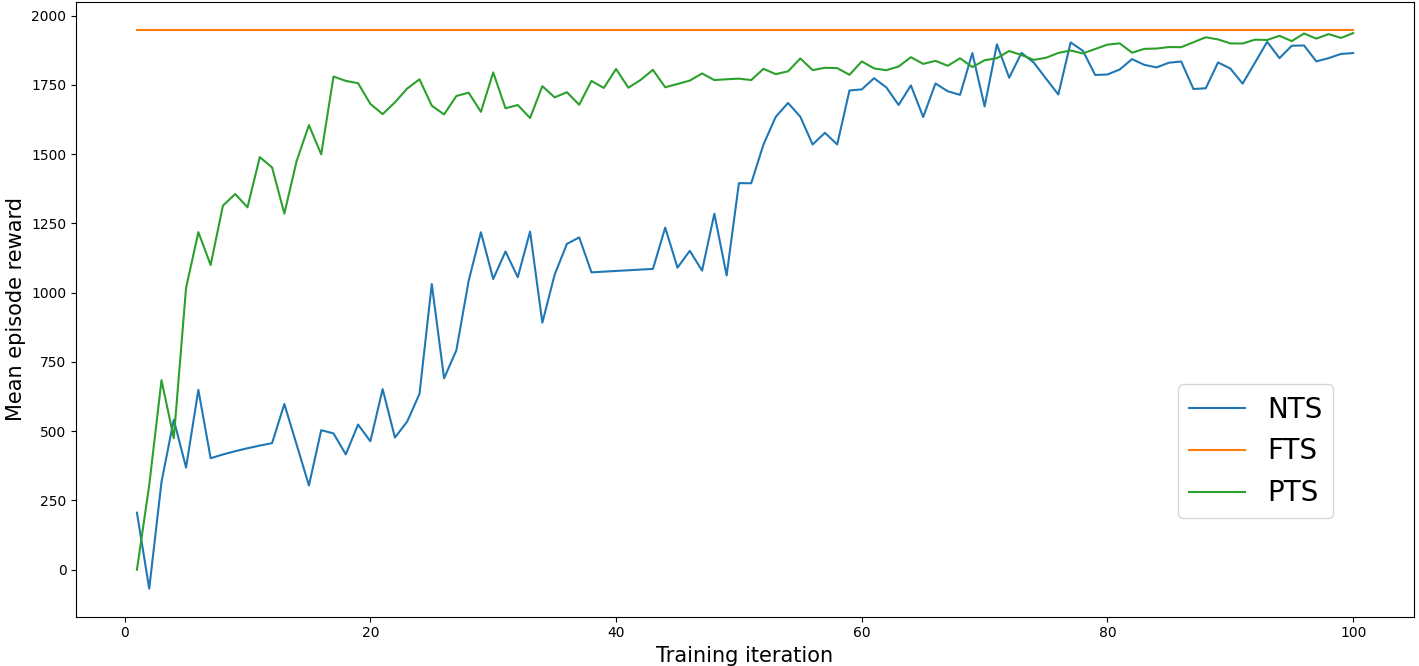
\includegraphics[width=0.46\textwidth]{figures/prahom_learning_curve.png}
    \caption{Average reward every training iteration (100 episodes) in the PBL environment for the NTS, PTS, and FTS cases\\ \phantom{X} \\}
    \label{fig:prahom_learning_curve}
\end{figure}

We also conducted a qualitative analysis of the resulting roles, links, and goals determined by PRAHOM after training.
%
For the PBL environment, we noticed roles being equivalent for agents are expected to act the same. Indeed, a Principal Component Analysis (PCA) presented in \autoref{fig:prahom_pca_analysis} of the agents' histories, shows most agents’ histories are in the left bottom zone (circled in red). It shows most pistons seem to act similarly as expected. One of the inferred sub-goals consists in having the ball in mid-way which is indeed coherent with expectations.
%
For the KAZ environment, we noticed acquaintance links due to each other's representation and two distinct roles: archers tend to move away from zombies, and knights tend to approach them. Despite the inferred sub-goals diversity, some indicate to have knights at the top while archers stay at the bottom as expected.
%
For the PPY environment, we noticed the output specifications indicate authority links between the leader predator and the simple predators. These are probably to be related to some inferred sub-goals that seem to indicate an approximated circling purpose.

\begin{figure}[h!]
    \centering
    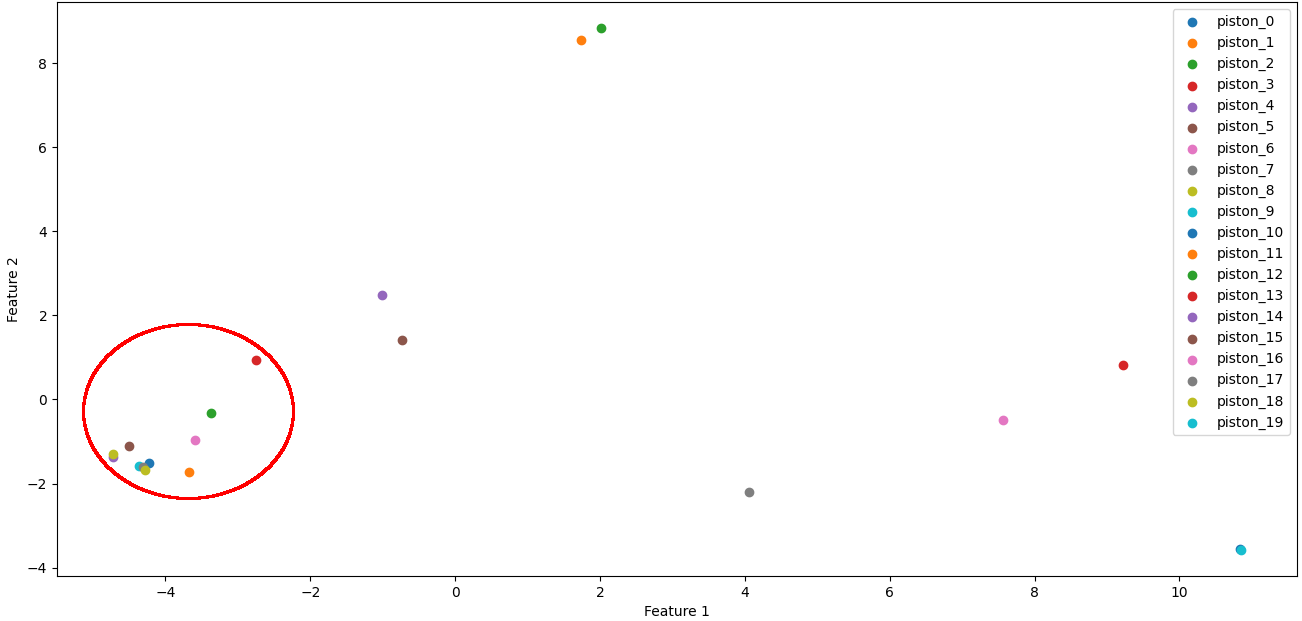
\includegraphics[width=0.45\textwidth]{figures/prahom_pca_analysis.png}
    \caption{PCA of the agents' histories in the PBL environment after training for the NTS case}
    \label{fig:prahom_pca_analysis}
\end{figure}



\section{Conclusion}

% résumer nos contributions et nos principales conclusions.

% importance d’améliorer l’explicabilité de l’IA dans les systèmes MARL et souligner l’impact potentiel de PRAHOM sur l’avancement du domaine.

% proposer des remarques finales et décrire les orientations des recherches futures afin d’explorer et d’affiner davantage notre algo.

% Multi-agent methods rely on the designer's knowledge to design a suitable MAS organization, but do not provide automatic means to determine the relevant organizational mechanisms only from the design requirements and the overall objective.
% MARL techniques have been successfully applied to automatically train agents to achieve a given objective without explicit characterization of emerging collective strategies.
% The PRAHOM's originality is to enrich a MARL process with an explicit organizational model towards a methodological objective to address these issues. It links the agents' policies (modeled in a Dec-POMDP) with $\mathcal{M}OISE^+$ through the process PRAHOM. Under the simplifying conditions of a group and a single social pattern, PRAHOM makes it possible to partially determine organizational specifications from joint histories and to constrain the training of policies in relation to organizational specifications.
% Additionally, we implemented the \emph{PRAHOM PettingZoo} wrapper as a proof of concept to apply PRAHOM.
% Finally, we applied our approach in four \emph{PettingZoo} environments to evaluate the impact during and after training. The performances obtained appear to be comparable to those known.

% Key point summary

Our main contribution is the PRAHOM algorithmic approach that aims to link MARL and agents' policies with the $\mathcal{M}OISE^+$ model leveraging on relations between joint-histories and organizational specifications. It seeks to determine organizational specifications from trained agents to help understand the agents' collective behavior. It also seeks to constrain the agents' training according to expected behaviors expressed as organizational specifications.
As a first implementation, \emph{PRAHOM PettingZoo Wrapper} is assessed in cooperative Atari games, where the inferred organizational specifications generally match the expected hand-crafted results.
Despite the implementation's limited functionalities, the first results showed that the PRAHOM approach can be used to constrain the resulting agents' policy space according to the specified organizational constraints. Additionally, we manually verified that some valuable organizational specifications are inferred from trained agents' histories.

% Perspectives
Even if PRAHOM is agnostic of any MARL algorithm, reconstructing the collective behaviors of agents a posteriori can prove difficult. Indeed, major perspectives to improve PRAHOM are inspired by hierarchical learning which contributes to better characterizing emerging strategies during learning.
Eventually, even though the first results obtained with LLM show it as a promising complementary help for PRAHOM, it may also bring out new ways for explaining collective behavior beyond its intended use.
% Ultimately, we also aim to improve the applicability of PRAHOM by developing dedicated interfaces built around PRAHOM making it more accessible to industrial and research contexts.


\section*{References}

\bibliographystyle{splncs04}

\bibliography{references}

\end{document}